%%%%%%%%%%%%%%%%%%%%%%%%%%%%%%%%%%%%%%%%%%%%%%%%%%%%%%%%%%%%%%%%%%%%%%%%%%%%%%%%
%% Plantilla de memoria en LaTeX para la ETSIT - Universidad Rey Juan Carlos
%%
%% Por Gregorio Robles <grex arroba gsyc.urjc.es>
%%     Grupo de Sistemas y Comunicaciones
%%     Escuela Técnica Superior de Ingenieros de Telecomunicación
%%     Universidad Rey Juan Carlos
%% (muchas ideas tomadas de Internet, colegas del GSyC, antiguos alumnos...
%%  etc. Muchas gracias a todos)
%%
%% La última versión de esta plantilla está siempre disponible en:
%%     https://github.com/gregoriorobles/plantilla-memoria
%%
%% Para obtener PDF, ejecuta en la shell:
%%   make
%% (las imágenes deben ir en PNG o JPG)

%%%%%%%%%%%%%%%%%%%%%%%%%%%%%%%%%%%%%%%%%%%%%%%%%%%%%%%%%%%%%%%%%%%%%%%%%%%%%%%%

\documentclass[a4paper, 12pt]{book}
%\usepackage[T1]{fontenc}

\usepackage[a4paper, left=2.5cm, right=2.5cm, top=3cm, bottom=3cm]{geometry}
\usepackage{times}
\usepackage[utf8]{inputenc}
\usepackage[spanish]{babel} % Comenta esta línea si tu memoria es en inglés
\usepackage{url}
%\usepackage[dvipdfm]{graphicx}
\usepackage{graphicx}
\usepackage{float}  %% H para posicionar figuras
\usepackage[nottoc, notlot, notlof, notindex]{tocbibind} %% Opciones de índice
\usepackage{latexsym}  %% Logo LaTeX
\usepackage{listings} %% Para que el codigo quede bonito

\title{Memoria del Proyecto}
\author{Nombre del autor}

\renewcommand{\baselinestretch}{1.5}  %% Interlineado

\begin{document}

\renewcommand{\refname}{Bibliografía}  %% Renombrando
\renewcommand{\appendixname}{Apéndice}

%%%%%%%%%%%%%%%%%%%%%%%%%%%%%%%%%%%%%%%%%%%%%%%%%%%%%%%%%%%%%%%%%%%%%%%%%%%%%%%%
% PORTADA

\begin{titlepage}
\begin{center}
\includegraphics[scale=0.8]{img/URJ_logo_Color_POS.png}

\vspace{1.75cm}

\Large
GRADO EN INGENIERÍA EN SISTEMAS AUDIOVISUALES Y MULTIMEDIA

\vspace{0.4cm}

\large
Curso Académico 2020/2021

\vspace{0.8cm}

Trabajo Fin de Grado

\vspace{2.5cm}

\LARGE
TÍTULO DEL TRABAJO EN MAYÚSCULAS

\vspace{4cm}

\large
Autor : Jorge De Pablo Martínez \\
Tutor : Dr. Gregorio Robles Martínez
\end{center}
\end{titlepage}

\newpage
\mbox{}
\thispagestyle{empty} % para que no se numere esta pagina


%%%%%%%%%%%%%%%%%%%%%%%%%%%%%%%%%%%%%%%%%%%%%%%%%%%%%%%%%%%%%%%%%%%%%%%%%%%%%%%%
%%%% Para firmar
\clearpage
\pagenumbering{gobble}
\chapter*{}

\vspace{-4cm}
\begin{center}
\LARGE
\textbf{Trabajo Fin de Grado}

\vspace{1cm}
\large
Título del Trabajo con Letras Capitales para Sustantivos y Adjetivos

\vspace{1cm}
\large
\textbf{Autor :} Jorge De Pablo Martínez \\
\textbf{Tutor :} Dr. Gregorio Robles Martínez

\end{center}

\vspace{1cm}
La defensa del presente Proyecto Fin de Carrera se realizó el día \qquad$\;\,$ de \qquad\qquad\qquad\qquad \newline de 202X, siendo calificada por el siguiente tribunal:


\vspace{0.5cm}
\textbf{Presidente:}

\vspace{1.2cm}
\textbf{Secretario:}

\vspace{1.2cm}
\textbf{Vocal:}


\vspace{1.2cm}
y habiendo obtenido la siguiente calificación:

\vspace{1cm}
\textbf{Calificación:}


\vspace{1cm}
\begin{flushright}
Fuenlabrada, a \qquad$\;\,$ de \qquad\qquad\qquad\qquad de 202X
\end{flushright}

%%%%%%%%%%%%%%%%%%%%%%%%%%%%%%%%%%%%%%%%%%%%%%%%%%%%%%%%%%%%%%%%%%%%%%%%%%%%%%%%
%%%% Dedicatoria

\chapter*{}
\pagenumbering{Roman} % para comenzar la numeracion de paginas en numeros romanos
\begin{flushright}
\textit{Dedicado a \\
mi familia / mi abuelo / mi abuela}
\end{flushright}

%%%%%%%%%%%%%%%%%%%%%%%%%%%%%%%%%%%%%%%%%%%%%%%%%%%%%%%%%%%%%%%%%%%%%%%%%%%%%%%%
%%%% Agradecimientos

\chapter*{Agradecimientos}
%\addcontentsline{toc}{chapter}{Agradecimientos} % si queremos que aparezca en el índice
\markboth{AGRADECIMIENTOS}{AGRADECIMIENTOS} % encabezado 

Aquí vienen los agradecimientos\ldots Aunque está bien acordarse de la pareja, no hay que olvidarse de dar las gracias a tu madre, que aunque a veces no lo parezca disfrutará tanto de tus logros como tú\ldots 
Además, la pareja quizás no sea para siempre, pero tu madre sí.

%%%%%%%%%%%%%%%%%%%%%%%%%%%%%%%%%%%%%%%%%%%%%%%%%%%%%%%%%%%%%%%%%%%%%%%%%%%%%%%%
%%%% Resumen

\chapter*{Resumen}
%\addcontentsline{toc}{chapter}{Resumen} % si queremos que aparezca en el índice
\markboth{RESUMEN}{RESUMEN} % encabezado

El lenguaje unificado modelado es en la actualidad la herramienta más utilizada en el modelado de software. No obstante, los diagramas y aspectos conceptuales del mismo pueden utilizarse para otros entornos, como el educativo.  

Este Trabajo de Fin de Grado tienen como objetivo desarrollar una aplicación web para uso docente y estudiantil a través de la cual alumnos de tempranas edades puedan aprender y familiarizarse con actividades que impliquen de alguna manera el entender y analizar diagramas para extraer información de estos. Todo esto se intentará hacer a través de gymkhanas y juegos para atraer de alguna manera el interés de usuarios más jóvenes.

La aplicación se ha desarrollado prácticamente en su totalidad con tecnologías \emph{OpenSource}, o en su defecto sobre software de empresas pero que cuentan con planes gratuitos para propuestas estudiantiles y/o pequeñas pruebas de concepto y por su puesto el acceso a esta debe ser totalmente gratuito. Entre esas tecnologías hay que destacar Python y Django, junto con Boostrap, HTML, css, y Git para el control de versiones. Se ha desplegado en la red de internet gracias a Heroku y por tanto se puede tener acceso a Gymkhana App desde cualquier parte del mundo, en cualquier momento del tiempo.

%%%%%%%%%%%%%%%%%%%%%%%%%%%%%%%%%%%%%%%%%%%%%%%%%%%%%%%%%%%%%%%%%%%%%%%%%%%%%%%%
%%%% Resumen en inglés

\chapter*{Summary}
%\addcontentsline{toc}{chapter}{Summary} % si queremos que aparezca en el índice
\markboth{SUMMARY}{SUMMARY} 
The Unified Modeling Language is currently the most widely used tool in software modeling. However, the diagrams and conceptual aspects of it can be used for other environments, such as education.

This End of Degree Project aims to develop a web application for teaching and student use through which students of early ages can learn and become familiar with activities that imply in some way understanding and analyzing diagrams to extract information from them. All of this will be attempted through gymkhanas and games to somehow attract the interest of younger users.

The application has been developed practically in its entirety with \emph{OpenSource} technologies, or failing that, with company software but which have free plans for student proposals and/or small proofs of concept and, of course, access to it must be be totally free. These technologies include Python and Django, along with Bootstrap, HTML, css, and Git for version control. It has been deployed on the internet thanks to Heroku and therefore Gymkhana App can be accessed from anywhere in the world, at any moment of time.


%%%%%%%%%%%%%%%%%%%%%%%%%%%%%%%%%%%%%%%%%%%%%%%%%%%%%%%%%%%%%%%%%%%%%%%%%%%%%%%%
%%%%%%%%%%%%%%%%%%%%%%%%%%%%%%%%%%%%%%%%%%%%%%%%%%%%%%%%%%%%%%%%%%%%%%%%%%%%%%%%
% ÍNDICES %
%%%%%%%%%%%%%%%%%%%%%%%%%%%%%%%%%%%%%%%%%%%%%%%%%%%%%%%%%%%%%%%%%%%%%%%%%%%%%%%%

% Las buenas noticias es que los índices se generan automáticamente.
% Lo único que tienes que hacer es elegir cuáles quieren que se generen,
% y comentar/descomentar esa instrucción de LaTeX.

%%%% Índice de contenidos
\tableofcontents 
%%%% Índice de figuras
\cleardoublepage
%\addcontentsline{toc}{chapter}{Lista de figuras} % para que aparezca en el indice de contenidos
\listoffigures % indice de figuras
%%%% Índice de tablas
%\cleardoublepage
%\addcontentsline{toc}{chapter}{Lista de tablas} % para que aparezca en el indice de contenidos
%\listoftables % indice de tablas


%%%%%%%%%%%%%%%%%%%%%%%%%%%%%%%%%%%%%%%%%%%%%%%%%%%%%%%%%%%%%%%%%%%%%%%%%%%%%%%%
%%%%%%%%%%%%%%%%%%%%%%%%%%%%%%%%%%%%%%%%%%%%%%%%%%%%%%%%%%%%%%%%%%%%%%%%%%%%%%%%
% INTRODUCCIÓN %
%%%%%%%%%%%%%%%%%%%%%%%%%%%%%%%%%%%%%%%%%%%%%%%%%%%%%%%%%%%%%%%%%%%%%%%%%%%%%%%%

\cleardoublepage
\chapter{Introducción}
\label{sec:intro} % etiqueta para poder referenciar luego en el texto con ~\ref{sec:intro}
\pagenumbering{arabic} % para empezar la numeración de página con números

La siguiente memoria recoge el trabajo realizado durante el desarrollo de Gymkhana App. Se trata de una aplicación web diseñada y orientada para que niños y niñas puedan disfrutar de sencillos juegos a la vez que aprender conceptos de lenguaje unificado modelado.

\section{Contexto}
\label{sec:seccion}
Gymkhana App es una aplicación web con simples juegos que consisten en la resolución de retos asociados a diagramas UML (lenguaje unificado modelado, de las siglas en inglés \emph{Unified Modeling Language}), o extracción de las respuestas a través del análisis de estos. 

La idea surge bajo la premisa de fomentar y ayudar en el desarrollo de habilidades como el seguimiento de flujo, pensamiento lógico, simplificación y análisis de situaciones complejas y la resolución de problemas mediante la división de estos en un conjunto de actividades estructurales que juntas forman una solución. 

Los mini-juegos consisten en resolución de sencillos enigmas que se resuelven combinando sus habilidades con diagramas UML. El nivel elegido en esta primera versión está orientado para niños de edades tempranas. También se quiere ofrecer la posibilidad de ser utilizado por el equipo docente para que estos mismos o cualquier contribuidor pueda crear, diseñar y aportar nuevos retos y juegos que puedan ser utilizados por toda la comunidad de la aplicación. 

El objetivo final de este proyecto trata de poder aportar una infraestructura en forma de aplicación de acceso público y muy sencilla de entender y manejar por los usuarios con el objetivo de divulgar y enseñar conceptos de UML y que, a al vez, los más jóvenes se familiaricen con estos últimos a través los sencillos juegos y retos que contiene Gymkhana App. 


\section{Estructura de la memoria}
\label{sec:estructura}

La memoria de este trabajo esta estructurada de la siguiente manera: 

\begin{itemize}
  \item \textbf{Capítulo 1. Introducción.} Hace una descripción básica del proyecto y se exponen las ideas principales del mismo. A parte, también especifica la estructura de la memoria. 
  
  \item \textbf{Capítulo~\ref{chap:objetivos}. Objetivos.} En este capítulo se describe el objetivo principal de este proyecto y también objetivos más específicos e hitos a alcanzar durante el desarrollo de la aplicación.
  
  \item \textbf{Capítulo~\ref{chap:estado}. Estado del arte.}. Capítulo dedicado a las tecnologías utilizadas durante el desarrollo de la aplicación. Se hace una pequeña introducción de las mismas y se explican características básicas y propiedades que hacen que se pueda y tenga sentido utilizarlas en el proyecto.
  
  \item \textbf{Capítulo~\ref{chap:diseño}. Diseño e implementación.} Se hace una descripción más profunda y técnica de la arquitectura del proyecto a nivel interno. Explicando detalladamente con ayuda de diagramas el diseño de la aplicación desgranando los módulos que la componen.
  
  \item \textbf{Apéndice~\ref{app:manual}. Manual de usuario.} Pequeño recorrido por la interfaz de usuario de la aplicación donde se muestran con imágenes los pasos a seguir para iniciar, resolver o subir nuevos retos en Gymkhana App. 
  
   \item \textbf{Apéndice~\ref{app:diagramas}. Ejemplos de diagramas UML.} En este anexo se describen brevemente ejemplos de cada uno de los diagramas UML que se explican la sección~\ref{sec:UML}, también se añaden imágenes de cada uno de ellos con el fin de aportar información gráfica.
\end{itemize}


%%%%%%%%%%%%%%%%%%%%%%%%%%%%%%%%%%%%%%%%%%%%%%%%%%%%%%%%%%%%%%%%%%%%%%%%%%%%%%%%
%%%%%%%%%%%%%%%%%%%%%%%%%%%%%%%%%%%%%%%%%%%%%%%%%%%%%%%%%%%%%%%%%%%%%%%%%%%%%%%%
% OBJETIVOS %
%%%%%%%%%%%%%%%%%%%%%%%%%%%%%%%%%%%%%%%%%%%%%%%%%%%%%%%%%%%%%%%%%%%%%%%%%%%%%%%%

\cleardoublepage % empezamos en página impar
\chapter{Objetivos} % título del capítulo (se muestra)
\label{chap:objetivos} % identificador del capítulo (no se muestra, es para poder referenciarlo)


\section{Objetivo general} % título de sección (se muestra)
\label{sec:objetivo-general} % identificador de sección (no se muestra, es para poder referenciarla)

El objetivo de este trabajo es desarrollar una aplicación web sencilla, limpia y clara enfocada para su uso por niños que aprendan y se familiaricen con el lenguaje unificado modelado y sus tipos de diagramas. También tendrá un apartado que te permita subir juegos y actividades que se integren en la misma plataforma, por tanto, también permite el uso por parte de un equipo docente.

Con esta aplicación web un equipo docente debería ser capaz de poder crear una serie de gymkhanas en forma de juegos y retos basados en diagramas UML que estudiantes de edades tempranas sean capaces de manejar, entender y poder moverse por la interfaz de la aplicación de manera sencilla. 

\section{Objetivos específicos}
\label{sec:objetivos-especificos}
El proyecto general se ha desglosado en los siguientes objetivos y tareas más específicas: 
\begin{itemize}
	\item Diseñar una aplicación web sencilla y limpia sobre \emph{localhost} que permita resolver retos compuestos por una pregunta relacionada directamente con un diagrama embebido en una imagen sobre la web y una repuesta.
	\item Permitir agrupar cuantos retos se deseen en juegos o gymkhanas y crear un menú de juegos donde puedas seleccionar de 1 a \emph{n} juegos.
	\item Hacer accesible la aplicación en diferentes idiomas, a través del sistema de internacionalización I18N. De esta manera podemos disponer de este proyecto tanto en castellano como en inglés de manera muy sencilla y ofreciendo a otros desarrolladores o contribuidores poder traducir la aplicación a otros idiomas de una manera estandarizada. 
	\item Crear un sistema de gestión de usuarios que gestione directamente la base de datos de la aplicación, que permita a estos usuarios la posibilidad de subir contenido a la aplicación en forma de retos y además puedan agrupar estos retos y/o los creados por otros usuarios de la app a juegos nuevos que se añadirán al panel principal común.
	\item Añadir sistema de puntuación a los retos, siendo estos puntos acumulables en los usuarios, y con un control de retos ya superados por un usuario a la hora de la asignación de puntos. 
	\item Despliegue de la aplicación y migración de base de datos a un portal web público para que tener acceso a la misma desde cualquier parte del mundo.
\end{itemize}


%%%%%%%%%%%%%%%%%%%%%%%%%%%%%%%%%%%%%%%%%%%%%%%%%%%%%%%%%%%%%%%%%%%%%%%%%%%%%%%%
%%%%%%%%%%%%%%%%%%%%%%%%%%%%%%%%%%%%%%%%%%%%%%%%%%%%%%%%%%%%%%%%%%%%%%%%%%%%%%%%
% ESTADO DEL ARTE %
%%%%%%%%%%%%%%%%%%%%%%%%%%%%%%%%%%%%%%%%%%%%%%%%%%%%%%%%%%%%%%%%%%%%%%%%%%%%%%%%

\cleardoublepage
\chapter{Estado del arte}
\label{chap:estado}
La aplicación web en la que se basa este proyecto se ha desarrollado con diferentes tecnologías gratuitas y de código abierto (\emph{Open Source}), pero la piedra angular sobre la que se apoya todo el proyecto es sobre el lenguaje unificado modelado. 

\section{UML: Unified Modeling Language} 
\label{sec:UML}

El lenguaje unificado modelado, también conocido por sus siglas en inglés UML, es el lenguaje de modelado de software más utilizado actualmente. 

El modelado de software es una parte esencial en todo el proceso de desarrollo del software. Al igual que en el plano análogo de la construcción de rascacielos, los planos, mapas del sitio y modelos físicos cumplen un papel esencial en la finalización con éxito del proyecto, en el desarrollo de software el lenguaje unificado modelado es necesario para asegurarse de que la funcionalidad del producto final es completa y correcta, de que satisface las necesidades del usuario final y que el diseño del programa admite los requisitos de escalabilidad, solidez, seguridad, expansibilidad y otras importantes características de un software. 

Se puede definir como un lenguaje gráfico que tiene como finalidad documentar, construir, especificar y en definitiva visualizar un sistema. Así mismo, también ofrece un estándar con el que definir un sistema o modelo. 

Es importante destacar que UML no es un lenguaje de programación ni es programación estructurada, pues UML es un lenguaje de modelado con el que se definen métodos y procesos, es decir el lenguaje que describe el modelo.

Desde fue presentado el primer estándar UML en 1997 (UML 1.1) hasta día de hoy ha evolucionado, en el momento de redactar esta memoria la OMT\footnote{Object Management Group \url{https://www.omg.org/}}, organización que respalda UML, tiene formalmente liberada la versión 2.5.1, que es sobre la cual este proyecto se ha desarrollado.
Naturalmente entre medias de han aparecido y varias versiones menores las cual han ido actualizando y corrigiendo hasta la versión que se utiliza actualmente. Desde el año 2004, UML es un estándar aprobado por la ISO (ISO/IEC 19501:2005 Information technology — Open Distributed Processing — Unified Modeling Language) y en el año 2012 se actualizó la norma dando lugar a la ISO/IEC 19505-1, la última versión disponible en este momento.

En UML se definen distintos tipos de diagramas, los cuales muestran diferentes aspectos del modelo representado. 
Los dos tipos principales de diagramas son: diagramas \emph{estructurales} y diagramas de \emph{comportamiento}. En la Figura 3.1 se puede ve un "metadiagrama" donde están ordenados jerárquicamente los diferentes tipos de diagrama. De la misma manera, en el Apéndice~\ref{app:diagramas} se dejan ejemplos brevemente explicados de cada uno de los tipos de diagramas que se comentan a continuación.

\begin{figure}
	\centering
	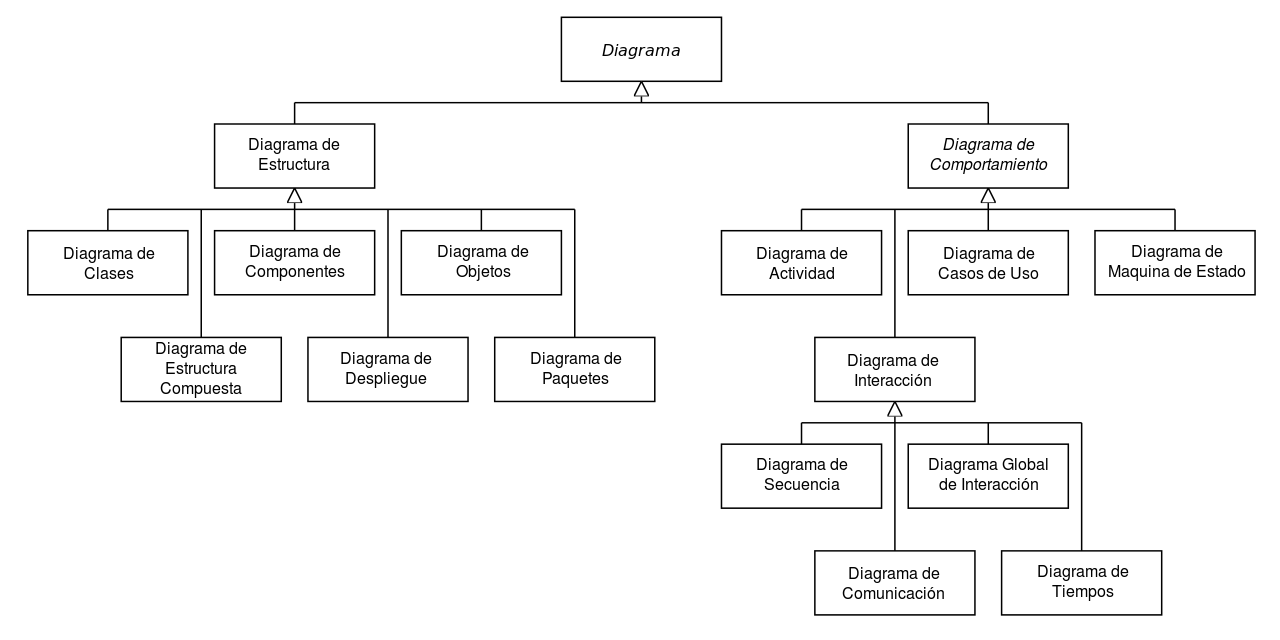
\includegraphics[width=16cm, keepaspectratio]{img/Uml_diagram.png}
	\caption{Jerarquía de diagramas en UML 2.2 (como diagrama de clases).}\label{fig:Uml_diagram}
\end{figure}

\subsection{Diagramas Estructurales}
Los diagramas estructurales muestran la estructura estática de los objetos en un sistema, es decir representan los elementos independientes del tiempo en un sistema. Los diagramas estructurales no muestran los detalles del comportamiento dinámico de un sistema, para ello existen los diagramas de comportamiento, sin embargo sí que pueden mostrar las relaciones entre los comportamientos definidos en la estructura.  

A continuación se describe brevemente cada uno de los diagramas pertenecientes a la familia de los diagramas estructurales que se muestran en la Figura 3.1: 

\subparagraph{Diagrama de clases}
Este tipo de diagramas proporciona los mecanismos para definir la estructura de un sistema estático. Muestra las clases del sistema, sus atributos, métodos y las relaciones y entre los objetos. 
\subparagraph{Diagrama de despliegue}
Esta clase de diagrama muestra la arquitectura de ejecución de un sistema. Incluyendo entornos de ejecución de hardware o software y el middleware que los conecta. Principalmente ayudan a entender y modelar la topología hardware de un sistema y como se despliega. 
\subparagraph{Diagrama de componentes} Los diagramas de componentes representan un sistema software dividido en componentes y muestra las dependencias entre los componentes. Son realmente útiles para ver qué componentes pueden compartirse entre sistemas o entre diferentes partes de un sistema.  
\subparagraph{Diagrama de objetos}
Este tipo de diagramas ofrece una vista parcial o completa de los objetos de un sistema. Es un gráfico de instancias que incluye objetos y datos. Estos diagramas están ligados a a los diagramas de clases, muestra el estado del sistema en un punto determinado del tiempo. 
\subparagraph{Diagrama de paquetes}
Representa las dependencias entre los paquetes que componen un sistema. Muestra como este está dividido en agrupaciones lógicas y las dependencias entre esas agrupaciones. Estos diagramas muestran la descomposición de la jerarquía lógica de un sistema.  
\subparagraph{Diagrama de estructura compuesta}
Esta clase de diagrama muestra la estructura interna de una clase y las relaciones e interacciones entre las distintas partes de la misma. Muestran el rol definido que tiene cada elemento y la estructura compuesta como el conjunto de esos elementos interconectados.
\subsection{Diagramas de Comportamiento}
Los diagramas de comportamiento muestran el comportamiento dinámico de un sistema, se puede describir como la serie de cambios que pueden existir en un sistema en un tiempo extraordinario.  
\subparagraph{Diagrama de actividad}
También conocidos como diagrama de flujo es la representación gráfica de un algoritmo o proceso. Representan flujos de trabajo paso a paso utilizando símbolos para representar cada uno de estos y flechas que conectan los símbolos para marcar el flujo de ejecución. 
\subparagraph{Diagrama de casos de uso}
Los diagramas de casos de usos describen los diferentes tipos de interacción que tiene alguien o algo con un determinado sistema, especificando el tipo de comunicación y comportamiento del mismo mediante la interacción con los usuarios y/u otros sistemas.
\subparagraph{Diagrama de interacción}
Este tipo de diagrama describen en detalle un determinado escenario de casos de uso. Ilustran la interacción entre el conjunto de objetos que cooperan en la realización de un proceso. También se pueden utilizar para representar secuencias ordenadas dentro de un sistema. Según las últimas versiones  de UML este diagrama se pueden clasificar en cuatro tipos principales de subdiagramas. 
\begin{itemize}
	\item Diagrama de colaboración. 
	\item Diagrama de secuencia. 
	\item Diagrama de tiempos. 
	\item Diagrama global de interacciones.  
\end{itemize}
Al igual que el resto de diagramas se hace una introspección más profunda en cada uno de estos diagramas en el Apéndice~\ref{app:diagramas}.
\subparagraph{Diagrama de máquina de estados}
Un diagrama de máquina de estados, conocidos en ocasiones como diagrama de estados modela el comportamiento de un objeto. Especifican la secuencia de eventos que sufre este determinado objeto durante su tiempo de ejecución. 

\section{Python}
Python es un lenguaje de programación interpretado, dinámico y multiplataforma con licencia de código abierto\footnote{Python Software Foundation License: \url{https://docs.python.org/3/license.html}}. Su máxima es hacer un lenguaje que sea fácilmente legible y con una empinada curva de aprendizaje. Python fue creado a principios de los 90s por Guido van Rossum en los Países Bajos, como curiosidad, saber que le debe su nombre gracias la afición que tenía su creador por el grupo de humoristas británicos Monty Python. 

\begin{figure}
	\centering
	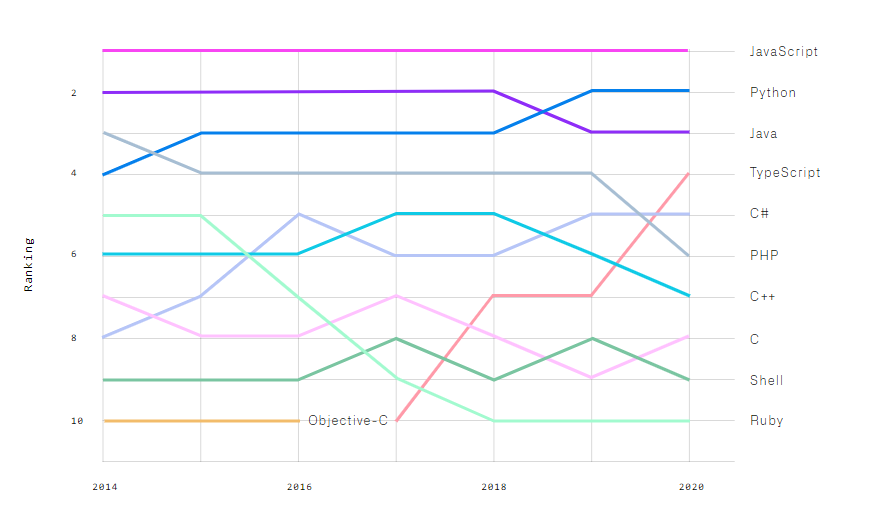
\includegraphics[width=18cm]{img/top_programing_languajes.png}
	\caption{Top uso de lenguajes de progrmación alojados en GitHub}
	\label{fig:Top_programming}
\end{figure}
%% (source:https://octoverse.github.com/#overview )

Dentro de sus características nos encontramos con que Python es: 
\begin{itemize}
	\item Interpretado: No es necesario que sea procesado por el compilador, se detectan errores en tiempo de ejecución 
	\item Multiparadigma: Soporta tanto programación funcional, como programación orientada objetos y también programación imperativa.  
	\item Tipado dinámico: Las variables se comprueban en tiempo de ejecución. 
	\item Flexible: No es obligatorio definir ni asignar variables antes de usarlas, es posible omitir parámetros, y sú única manera de definir la estructura del código en mediante indentación.
	\item Multiplataforma: Puede ejecutarse tanto en Linux, como Windows como macOS. 
\end{itemize}


Gracias a la versatilidad y fácil acceso a este lenguaje ha provocado que en los últimos años se haya vuelto muy relevante haciendo que sea uno de los principales y más importantes lenguajes de programación usados hoy en día. Como se puede ver en la Figura 3.2.
Actualmente su última versión estable es Python 3.9, pero este proyecto ha sido desarrollado usando la versión 3.7.3, ya que es una de las más populares y con más usuarios en activo. También cuenta con una versión anterior muy popular, Python 2, que es fue considerada \emph{"deprecated"} el 1 de enero de 2020. 

  
\section{Django}
Django es un framework de desarrollo web gratuito, de código abierto y escrito en Python. Fue lanzado en Julio de 2005 y comparte objetivos generales con Python buscando fundamentalmente poder desarrollar sitios web complejos de manera sencilla y accesible para el mayor número de personan posibles. Django funciona bajo Python, es decir, que para poder trabajar con Django es necesario tener instalado Python. 

Un framework, traduciéndolo al castellano, viene a ser un marco de trabajo, una especie de ecosistema formado por un  conjunto de herramientas, librerías y buenas prácticas para crear aplicaciones, en este caso para desarrollar aplicaciones web. 

El framework de Django en concreto nos permite crear sitios web con un cierto grado de complejidad de manera rápida y sencilla. Muchas de las tareas al realizar sitios web suelen ser repetitivas pesadas y comunes en la mayoría de casos, Django viene a facilitar la realización de estas tareas. 

\subsection{Modelo Vista Controlador (MVC)}
Modelo-vista-controlador es un patrón de arquitectura de software, este patrón consiste en dividir este patrón en tres grandes módulos: modelo, vista y controlador. 

\begin{itemize}
 \item Modelo: Se encarga de gestionar los datos, normalmente de obtener información de una base de datos. 
 \item Vista: Se encarga de mostrar la información al usuario y las interacciones del mismo con el sistema. 
 \item Controlador: Gestiona todas las comunicaciones que existen entre la vista y el modelo. 
\end{itemize}

Esta división en módulos tiene como ventaja que hace las aplicaciones más funcionales, sostenibles, y escalables. Otros muchos grandes frameworks de desarrollo web usan este modelo y Django básicamente también, pero llaman a su modelo de manera diferente. La filosofía sigue siendo la del modelo-vista-controlador pero se llama Model Template View, lo que hace es susttuir las vistas por un módulo que llama Template, o plantilla en castellano, el controlador de Django viene a ser el módulo Views y el Model sigue siendo el modelo.

\section{Git} 
Git es un sistema de control de versiones gratuito y de código abierto diseñado para manejar cualquier tipo de proyecto, tanto en pequeños como los muy grandes con gran velocidad y eficiencia. Vino desarrollado por la mano de Linus Toval, famoso por iniciar el desarrollo del kernel del sistema operativo Linux. 

Git es fácil de aprender y ocupa poco espacio con un rendimiento increíblemente rápido. Su objetivo es facilitar el desarrollo y mantenimiento de código fuente tanto de forma individual como, sobre todo, de trabajo en equipo. Te permite, crear varias ramas de desarrollo y provee de herramientas para poder unir y estas ramas además de guardar un registro de todos los cambios que sufran los archivos. 

Este software es multiplataforma, se puede instalar tanto en Linux, como en Windows y macOS. Se puede utilizar cualquier tipo de lenguaje de programación sobre el archivo del que se desea hacer control de versiones, ya que Git no se fija en el contenido sino en la diferencia de este contenido a lo largo del tiempo y en las diferentes ramas. 

Los repositorios de código que usan Git como control de versiones no necesariamente tienen que estar alojados en un repositorio de internet, pero lo más habitual y práctico es que sí lo esté. Existen numerosas plataformas que te permiten alojar repositorios de código fuente e interactuar con las herramientas de Git como GitLab o Gogs, que son de código abierto y gratuitas o siios como CodeComit que perteneze a AWS\footnote{Amazon Web Services} y por tanto es de dominio privado. En este proyecto durante su desarrollo se ha utilizado Git para el control de versiones alojando el repositorio en GitHub, que es el otro sitio más de código abierto para alojar proyectos, es gratuita y típicamente se almacenan los repositorios de forma pública.

\section{Boostrap}
Boostrap es un framework de código abierto y multiplataforma que contiene bibliotecas y herramientas para el diseño de aplicaciones web. Contiene plantillas de diseño con tipografía, formularios, botones, menús de navegación y otros elementos basado en HTML y CSS, así como extensiones de JavaScript adicionales. Fue desarrollado por Mark Otto y Hacob Thornton como marco de trabajo para fomentar las herramientas internas de Twitter, en 2011 se liberó como código abierto bajo una licencia MIT License.

Boostrat tiene soporte relativo para HTML5 y CSS3, pero es compatible con la mayoría de los navegadores web. Desde su versión 2.0 soporta diseños wen adaptables. Esto significa que eñ diseño de la web se ajusta dinámicamente en función del display del que disponga el dispositivo donde se esté visualizando, esta tecnología también se conoce como responsive cuando hablamos de desarrollo web. 

Este framework web sólo se ocupa del desarrollo del front-end, es decir de la parte que ve e interactua el usuario directamente. Integrando este framework con el modelo-vista-controlador de Django, explicado anteriormente en el punto 3.3.1 de este documento podemos enmarcarlo dentro del módulo Template de Django, pudiendo dividir así la parte funcional y práctica del proyecto de la parte del diseño relegándola en Boostrap. 

\section{Heroku}
Heroku es una plataforma que ofrece servicios de computación en la nube que soporta distintos lenguajes de programación. Fue desarrollada en 2007 con el objetivo de soportar la únicamente el lenguaje de programación Ruby, pero poco a poco extendió su soporte para otros lenguajes como Node, Java, PHP y Python entre otros. También soporta servicios de bases de datos tanto MongoDB como Redis o PostgreSQL, tanto como parte de la plataforma como servicio independiente. Además de esto tiene integración con Git, que dentro de Heroku será quien maneje los repositorios de las aplicaciones subidas por los usuarios. 

El modelo de arquitectura de Heroku se basa en Dynos, que son unidades de capacidad de cómputo basadas en contenedores Linux que hay dentro de la plataforma. Cada Dyno está aislado del resto por lo que se pueden desplegar entornos y procesos en cada uno de estos sin que se vean afectado otros. Esto otorga a estas pequeñas máquinas unitarias las siguientes características: 
\begin{itemize}
	\item Elasticidad y crecimiento: La cantidad de Dynos se puede cambiar en cualquier momento. 
	\item Tamaño: Puedes elegir diferentes unidades de memoria y procesamiento en cada máquina. 
	\item Routing: Internamente se conoce la ubicación de los Dynos y por tanto redirigen el tráfico eficientemente. 
	\item Seguimiento: Existe un manejador de Dynos, el cual está continuamente monitorizando sus servicios, en caso de que alguno falle este nodo es eliminado y levantado nuevamente. 
	\item Distribución y redundancia. Estas unidades de procesamiento al estar aisladas implica que si existen fallos en la infraestructura de una de ellas otras no se verán afectadas y en consecuencia tampoco sus servicios. 	
\end{itemize}

Heroku, a diferencia de otras tecnologías vistas en este documento, no es un servicio puramente gratuito, ya que es propiedad de Salesforce, una gran empresa estadounidense de software bajo demanda. No obstante, su unidad de cómputo más básica es de uso gratuito. Con una de estas unidades o Dynos es suficiente para experimentar, poder trabajar en pequeñas aplicaciones y en pruebas de concepto. Todas estas características convierten e a este servicio en un entorno perfecto para desplegar una aplicación web pequeña o mediana de manera gratuita para que esté disponible en cualquier parte del mundo. 
\subsection{Heroku PostgreSQL}
Heroku ofrece la base de datos PostgreSQL de código abierto en forma de Heroku Postgres. 

Heroku Postgres es una de las soluciones que más usan los desarrolladores en los proyectos de la plataforma. Ofrece todas las ventajas de utilizar PostgreSQL como escalabilidad, acceso a un sistema de administración, seguridad, una alta concurrencia y otras características que se detallan de manera más profunda en el punto 3.8. 

Los planes de precio dentro que Heroku ofrece a sus usuarios para este servicio pasan por una gran variedad de precios pero cuenta con un plan gratuito para desarrolladores que permite probarlo sin ningún riesgo con un tamaño y características más que suficientes para pequeños proyectos o pruebas de concepto sencillas. 

\section{SQLite 3}
SQLite es un sistema de gestión de bases de datos relacional de código abierto.  A diferencia de los sistemas de gestión de bases datos cliente-servidor la biblioteca SQLite es una parte integral de la programa que enlaza y no un proceso independiente del mismo. Esto hace que la latencia sea más reducida, y las comunicaciones entre procesos y funciones son más eficientes. 

SQLite nació ne el año 2000, fue creado por D. Richard Hipp Y su objetivo era diseñar un sistema de gestión de bases de datos relacional que permitiera ejecutar programas sin la necesidad de instalar un sistema de gestión de bases de datos. 

Sus primeras versiones se caracterizaban por contener la base de datos en un espacio en disco relativamente pequeño y está contenida en un solo archivo. En su versión 3, SQLite admite bases de datos de hasta 2 Terabytes de tamaño. 

Este sistema de gestión de bases de datos soporta funciones SQL definidas por los usuarios, y tiene otras ventajas como una amplia compatibilidad con diferentes plataformas como Windows, Linux, Android, MacOS e iOS. También es compatible con caso todos los lenguajes de programación y proporcionando API útiles para ellos. Por defecto es la base de datos que viene configurada para proyectos de Django, por su ligereza, independencia de paquetes externos y la eficiencia de sus procesos es ideal para pruebas de concepto en proyectos pequeños, pero es difícil de escalar y al no presentar el estándar cliente-servidor tiene limitaciones en cuanto al formato y la sintaxis, y no presenta muchas funciones de seguridad.

\section{PostgreSQL}
PostgreSQL, también llamado Postgres, es un sistema de gestión de bases de datos relacional orientado a objetos y de código abierto. Este proyecto de código abierto no es gestionado por una persona o empresa, sino que lo mantienen una comunidad de desarrolladores que trabajan de forma altruista y libre, el PGDG.\footnote{PostgreSQL Global Development Group}

Entre las características principales de este sistema de gestión de bases de datos se encuentran: 
\begin{itemize}
	\item Alta concurrencia: Permiten que varios usuarios o procesos accedan a la misma tabla sin necesidad bloqueos. 
	\item Amplia variedad de tipos nativos: PostgreSQL provee nativamente soporte para diferentes tipos de datos como texto ilimitado, direcciones IP o MAC o CIDR, arrays, números de precisión arbitraria e incluso figuras geométricas (con variedad de funciones asociadas). Adicionalmente permite que los usuarios puedan crear sus propios ipos de tos , que pueden ser  perfectamente indexables. 
	\item Otrás características deseables en un gestor de bases de datos, como claves foráneas (\emph{foregin keys}), disparadores, herencia de tablas, integridad transaccional, seguridad y escalabilidad.  
\end{itemize}
Las ventajas que ofrecen todas esté gestor de base de datos son básicamente seguridad e integridad en términos generales en la BD\footnote{Base de Datos}, un buen sistema de transacciones y respaldos y una conexión a sistema de gestión de base datos. Desafortunadamente no cuenta con gestor de errores, or tanto es difícil conocer el estado de los errores o corregirlos. 

Como ya vimos en el punto 3.6, PostgreSQL cuenta con un paquete propio integrado en Heroku que permite utilizar este sistema de gestión de bases de datos junto con el almacenamiento de los mismos en servicios virtualizados de manera gratuita en algunos de sus planes.  

\section{Visual Studio Code}
Visual Studio Code es un editor de código fuente lanzado en 2015 y desarrollado por Microsoft. Es un editor multiplataforma compatible con Windows, Lunux, MacOs y ahora cuenta también con una versión web. 

Soporta prácticamente cualquier lenguaje de programación conocido, resaltando la sintaxis del mismo de manera personalizada, ofrece sugerencias de sentencias y variables y finalización inteligente de código, integración con la shell y gestor de archivos interno. Incluye soporte para depuración, control de versiones integrado con Git. Además gracias a la gran comunidad de desarrolladores existen infinidad de \emph{pluggins} muy fácilmente instalables que añaden funcionalidades realmente útiles a la hora de programar, depurar, integrar o desplegar código. 
Es un software gratuito y de código abierto pero la descarga oficial esta bajo software privativo de Microsoft. 

Visual Studio Code recopila datos de uso y los envía a Microsoft, aunque esto se puede desactivar, y por la natuuraleza open-source de la aplicación se puede ver exactamente que clase de datos se recopilan y envían. Los datos pueden ser compartidos entre Microsoft, sus filiales y las autoridades según lo firmado conformemente en la declaración de privacidad. 

\section{WSL 2}
Windows Subsystem for Linux (WSL) es una capa de compatibilidad entre sistemas desarrollada por Microsoft con el objetivo de poder correr ejecutables de Linux nativamente en Windows 10 y Windows Server. En 2019 se lanza la versión 2 de WSL incluyendo cambios importantes, como el uso real del kernel de Linux. 

WSL ofrece una interfaz que simula el kernel de Linux sobre Windows sin necesidad de instalar un SO\footnote{Sistema Operativo} en particiones de disco y sin necesidad de crear una máquina virtual que tenga que emular hardware. Establece un espacio de usuario GNU\footnote{GNU es un sistema operativo de tipo Unix, así como una gran colección de programas informáticos que componen al sistema, desarrollado por y para el Proyecto GNU y auspiciado por la Free Software Foundation.} donde instalar un sistema base como Ubuntu, Debian o Kali Lunux. Dicho entorno no contará con interfaz gráfica(a no ser que tenga ayuda de aplicaciones gráficas como un servidor X11) sino que se accedera a ella mediante una shell de tipo Bash\footnote{Bash (Bourne-again shell) es una popular interfaz de usuario de línea de comandos, específicamente un shell de Unix; así como un lenguaje de scripting}. 

Para acceder al hardware y al sistema de archivos se hace uso directo del sistema de archivos en Windows y partes del hardware como el hardware de red e incluso su infraestructura como los puertos. Este uso compartido del sistema hace que haya gran interoperabilidad entre ambo. Esto permite incluso desarrollar software sobre Linux, en un sistema Windows con sus aplicaciones propias como Visual Studio, hacer que ejecute el código en un entorno Linux con sus respectivos paquetes de software y acceder al programa o aplicación desarrollado a través de un puerto de red en un navegador de Windows con relativa facilidad. 

\section{Diagrams.net}
Diagrams.net, anteriormente conocido como draw.io, es un software de código abierto de dibujo gráfico, pensado especialmente para la creación y dibujado de diagramas.

Esta desarrollado en HTML5 y JavaScript, es multiplataforma y esta disponible en aplicación web\footnote{https://app.diagrams.net/}. A parte de ser muy intuitiva y fácil de manejar no requiere inicio de sesión o registro. Permite exportar los diagramas o dibujos a gran cantidad de formatos como .PNG, .PDF, .SVG y .JPEG. Y se puede integrar con servicios de almacenamiento \emph{onCloud} como Google Dive, Dropbox o OneDrive (para estas funcionalidades si es necesario registrarse) y cuenta con un complemento para integrar la aplicación web en Visual Studio Code. Lo cual simplifica el poder hacer diagramas UML paralelamente al desarrollo de un software.


%%%%%%%%%%%%%%%%%%%%%%%%%%%%%%%%%%%%%%%%%%%%%%%%%%%%%%%%%%%%%%%%%%%%%%%%%%%%%%%%
%%%%%%%%%%%%%%%%%%%%%%%%%%%%%%%%%%%%%%%%%%%%%%%%%%%%%%%%%%%%%%%%%%%%%%%%%%%%%%%%
% DISEÑO E IMPLEMENTACIÓN %
%%%%%%%%%%%%%%%%%%%%%%%%%%%%%%%%%%%%%%%%%%%%%%%%%%%%%%%%%%%%%%%%%%%%%%%%%%%%%%%%

\chapter{Diseño e implementación}
\label{chap:diseño}


\section{Arquitectura general} 
\label{sec:arquitectura}

La aplicación web Gymkhana App se ha desarrollado en Django con su estructura típica basada en el modelo-vista controlador como se ve en la figura~\ref{fig:arquitectura}, en esta figura las lineas sólidas muestran una relación directa entre los elementos y las rayadas una asociación indirecta. Dentro de este modelo  la vista será la capa que se presente y con la que interactua el usuario, compuesta por los diferentes tipos de plantillas o Templates como los conoce Django. El modelo es quien se encarga de gestionar los datos, es quien tiene comunicación directa con la base datos y maneja toda la información que entra y sale de esta. El controlador es quien maneja las comunicaciones entre los dos anteriores módulos y el único que tiene conexión directa con el resto de módulos, se encarga de recibir las peticiones del módulo de vistas, gestionar internamente estas peticiones y decidir que hacer en base a la información recogida consultando en cualquier caso los datos que considere necesarios del modelo. 

\begin{figure}
	\centering
	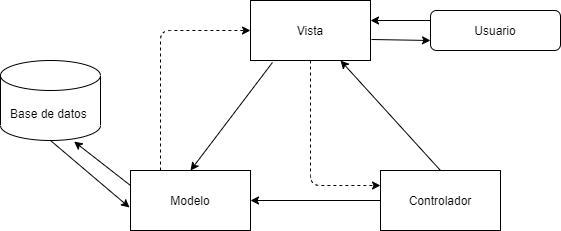
\includegraphics[width=12cm, keepaspectratio]{img/model-vista-controlador.png}
	\caption{Estructura de las relación modelo-vista-controlador.}\label{fig:arquitectura}
\end{figure}

\section{Módulo Vistas-Controlador}
Este módulo es el encargado de recibir y gestionar las peticiones recibidas desde el módulo Templates, gestionarlas, consultar con el módulo Models y preparar las respuestas para el usuario. Django dispone de herramientas muy útiles para la gestión y respuesta de peticiones web, de tal manera que definir las funciones del servidor cada vez que un usuario accede a una URL y generar las respuestas es limpio, sencillo, escalable. 
Las URL y como se gestionan las respuestas se define a continuación: 

\begin{itemize}
	\item \textbf {/ (Home)}: Como muchas otras aplicaciones que existen, cuando se introduce la URL con el nombre completo del dominio sin añadir ningún directorio tras este, se redirige con esta petición a la página principal o home, donde se simplemente se puede ver dos botones grandes que te permiten o bien iniciar sesión y registrarte o bien iniciar Gymkhana App. 
	\item \textbf {/start}: Cuando inicias la Gymkhana desde el home te lleva automáticamente a esta dirección, donde primero este módulo comprueba si existen juegos disponibles en la base de datos, y si es así los muestra. El usuario puede elegir uno de estos juegos y enviar una petición GET con el identificador del juego elegido. 
	\item \textbf {/challenge}: Cuando se accede a este directorio se recoge la petición GET del usuario con el juego elegido, y si vienes de un reto anterior o acaba de empezar el juego. Así podemos elegir cual de los diferentes retos que componen un juego mostrar, siempre comprobando que todos los datos existan en la base de datos para evitar posibles errores. Una vez elegido el reto a mostrar se le muestra a el reto donde el usuario debe introducir la respuesta al mismo para poder avanzar. 
	\item \textbf {/response}: Una vez el usuario ha rellenado la repuesta al reto se envía una petición tipo GET con la información contenida del reto al que pertenece, el juego, si ha habido una reto del mismo juego anterior y la respuesta al reto. En caso de ser correcta el servidor redirigirá al usuario bien al nuevo reto, si se está jugando a un juego con varios retos, o una pantalla en la que indica que ha finalizado correctamente el juego y desde ahí el usuario podrá regresar al menú principal para poder elegir otros juegos, o repetir el mismo. También en cada response se analizará si el usuario que está jugando está registrado y le añadirá a ese usuario la puntuación que de dicho reto, pero solo en caso de que no lo halla completado anteriormente. Por otro lado, si la respuesta no es correcta, enviará al usuario a una pantalla donde se indica que la respuesta es incorrecta y te dejará volver a intentar el reto o salir al menú de juegos.
	\item \textbf {/accounts}: Esta dirección funciona de una manera un poco diferente. Para el inicio de sesión, modificación de contraseñas y cierre de la misma en la aplicación se ha decidido utilizar un módulo ya implementado de Django que gestione correctamente estas peticiones. Este módulo se le conoce como "Django’s authentication system" y esta dentro de la configuración por defecto de Django. Una vez accedemos a esta dirección el usuario deberá ingresar su nombre de usuario y contraseña para poder continuar. En caso de ser correcto redirigirá al usuario a su perfil. Cuando el usuario decida cerrar la sesión se le redirigirá al home de la aplicación. 
	\item \textbf {/profile}: Si te registras en la aplicación exitosamente podrás acceder a tu perfil de usuario a traves de una petición GET en esta dirección. Básicamente aquí se muestra la información del usuario, como el nombre o el acumulado de sus puntos. También se podrá acceder a /start para comenzar a jugar. Desde este punto el usuario que ha iniciado sesión puede acceder a los módulos para crear retos y juegos 
	\item \textbf {/create challenge}: En esta dirección primero comprueba que el usuario esté registrado y si es así se le muestra un formulario con los campos necesarios que componen un reto. Para poder continuar desde este punto habrá que haber rellenado correctamente todos los datos del formulario y pulsar el botón de subir reto. 
	\item \textbf {/upload challenge}: La activación de botón mencionado en el apartado anterior enviara los datos del formulario mediante una petición POST. En este punto se revisa que los campos requeridos hayan sido rellenados correctamente y en caso afirmativo se guarda este reto en base de datos.  
	\item \textbf {/create game}: Al igual que para crear un reto, se accede a este módulo desde la página del usuario, una vez se haya registrado. En este caso una vez se haya accedido se presenta un formulario para poder crear un juego. Como los juegos son simples colecciones de retos, aquí se le muestra al usuario un listado con los retos subidos para que seleccione uno o varios retos. La única forma de avanzar desde este punto será pulsando el botón de subir juego con el formulario correctamente cumplimentado. 
	\item \textbf {/upload challenge} Para terminar la subida de un juego se envían los campos del formulario contenidos en una petición POST que será la se espera recibir aquí. En caso de que todos los campos requeridos existan y sean correctos subirá el juego a la base de datos de la aplicación Gymkhana App.
	
\end{itemize}

Django cuenta con muchas funciones y respuestas que vienen ya integradas, como por ejemplo poder responder a peticiones que provocan errores genéricos como tipo HTTP 404 (Not Found) entre otros, de esta manera todas las peticiones que se hacen al servidor en caso de encontrar la información requerida en la base de datos la aplicación captura este error y devuelve un ERROR 404 genérico de Django, que aparte hace terminar el resto de procesos en curso, haciendo a la aplicación mucho más robusta ante errores. 


\section{Módulo Templates-Vistas}
El módulo de Templates es el que forma la interfaz de usuario de la aplicación. Cada vista de la aplicación, o página que el usuario acaba visualizando está compuesta por un template o plantilla HTML sobre la que se aplica un estilo con CSS. Trabajar con plantillas en Django hace que la aplicación sea escalable y el código quede ordenado. En muchos casos la plantilla es reutilizable si se parametrizan adecuadamente, a su vez, la capa de estilo esta muy bien aislada gracias a Boostrap, de manera que se puede separar muy bien la parte programática del desarrollo de la parte encargada del diseño y el estilo evitando así tener que aplicar estilo a cada una de las páginas implicadas en el desarrollo. 

La aplicación de Gymkhana App se compone de las siguientes views: home, start, challenge, succes y wrong, login, profile, create challenge y create game
\subparagraph{Home}
Es la página principal que el usuario ve cuando accede a la web. Se limita a una presentación sencilla y limpia del proyecto, con un botón bien visible al usuario que será el que le permita avanzar y adentrarse en Gymkhana App. 
\subparagraph{Start}
Esta página actúa de forma de menú y muestra los juegos que hay disponibles en la aplicación, los lista ordenadamente de manera descendientes, y cada juego tiene un botón con el que él usuario puede interactuar, pulsando el mismo se accede a dicho juego.  
\subparagraph{Challenge} 
En esta página muestra un único reto, que se compone de un nombre o título, una pregunta y una imagen con un diagrama UML que debe estar relacionado con el reto. Esta vista tiene también un campo que el usuario debe rellenar con la respuesta planteada al reto y un botón par enviar la petición que más tarde procesará el módulo Vistas-Controlador.
\subparagraph{Success}
Una vez enviada la respuesta a un reto, si eta es correcta te redirigirá a esta página donde puedes ver un texto dando la enhorabuena al usuario. Dependiendo del juego te mostrará un botón para volver al menú de juegos o al siguiente reto si el juego estaba compuesto por varios. 
\subparagraph{Wrong}
En contraposición a la anterior plantilla, esta mostrará al usuario un comentario haciéndole saber que la respuesta no es correcta, pero también animándolo a que lo vuelva a intentar. Esta plantilla solo mostrará dos botones, uno para volver a intentar el reto que ha fallado y otro para volver al menú de juegos en caso de que el usuario desista y de por perdido el reto. 

\subparagraph{Login}
Tiene la estructura de cualquier pagina de inicio de sesión tradicional, donde el usuario debera introducir su nombre y contraseña para acceder. Como diferencial al resto de sitios web, Gymkhana App no ofrece en esta página la opción de crear un usuario, ya que un usuario registrado tiene la capacidad de hacer inyecciones en la base de datos y subir contenidos como imágenes. Por tanto y por motivos de seguridad, la potestad de creación de usuarios queda relegada solo al administrador de este proyecto que, en todo caso, proporcionara las credenciales de registro a quien considere necesario.   

\subparagraph{Profile} Una vez el usuario esté registrado tendrá acceso a esta página, donde podrá ver información del usuario, como su nombre en la aplicación y los puntos que ha obtenido. Además desde este punto tendrá acceso a las dos siguientes views: create challenge y create game

\subparagraph{Create Challenge} En esta página se podrá ver un formulario con los campos que debe rellenar un usuario para poder subir el reto. Los campos son los siguientes:
\begin{itemize}
	\item \textbf {nombre}: Nombre o título deseado para el reto.
	\item \textbf {pregunta}: Será la cuestión a la que los jugadores deban responder para poder completar el desafío.
	\item \textbf {solución}: La respuesta o solución correcta que se espera por parte del jugador para poder completar el reto.
	\item \textbf {tipo de diagrama}: En este campo se despliega una lista con todos los tipos de diagramas UML para que el usuario que está subiendo el juego seleccione el tipo de diagrama al que pertenece el usado en el reto.
	\item \textbf {imagen}: Un campo que permite al usuario abrir el explorador de archivos de su sistema operativo para poder subir una imagen, en concreto se debe subir la imagen del diagrama UML asociado al reto. 
	\item \textbf {puntos}: Valor que se le quiere dar en puntos al reto.
\end{itemize}	

\subparagraph{Create Game} Al igual que la anterior esta página mostrará un formulario que se deber rellenar para poder crear juegos. 
\begin{itemize}
	\item \textbf {título}: Nombre o título deseado para el juego.
	\item \textbf {retos}: Se muestra una lista con todos los retos subidos a la plataforma, tanto los creados por ese usuario como los creados por otros. El usuario que cree un juego puede elegir uno o tantos como considere para formar un juego. 
\end{itemize}	


Todas estas páginas han sido construidas sobre una base genérica común que usan todas las plantillas. Esta base común permite contener la información de todas las vieews mencidonadas anteriormente, además de la cabecera o header y el pie de página o footer. En la cabecera hay dos enlaces ocultos que redirigirán al usuario bien a la página principal de la aplicación Gymkhana App, o a la web oficial de la organización UML. En el pie de página se muestra información relativa a la ETSIT como localización y enlaces ocultos para poder visitar la cuenta de Twitter, y la web oficial de la ETSIT. También aparece la licencia de uso de la plantilla de Boostrap elegida

\subsection{Internacionalización}
Django también ofrece de manera relativamente sencilla la posibilidad de añadir internacionalización a las plantillas. Este proceso consiste en traducir todo el texto que aparece en las plantillas. 

En este proyecto, el idioma original que se eligió para desarrollar las plantillas fue el inglés, pero con el proceso de internacionalización también está disponible en castellano. La idea básica de la internacionalización o I18N es marcar aquellas cadenas de texto que deben ser traducidas. Estas cadenas se guardan en un diccionario, donde se añade la traducción al idioma o idiomas deseados, de esta manera cuando un usuario seleccione un idioma, mostrará estas cadenas de texto marcadas en el lenguaje que le corresponda al usuario. 

En el diccionario aparte de todas las cadenas de texto que se muestran en las diferentes plantillas, también están guardadas las respuestas a los retos. Esta es la única manera de poder procesar las respuesta de los usuarios en diferentes idiomas y comprobar que coinciden con la respuesta de un reto concreto. 

De la misma manera, para poder traducir las imágenes de los diagramas UML que se muestran, cada diagrama tiene que estar disponible en dos idiomas diferentes, es decir cada diagrama está representado por dos imágenes, una en inglés y otra en castellano, así se seleccionará la imagen correspondiente dependiendo del idioma del usuario. 

\section{Módulo Models-Modelo}
Este módulo es el que gestiona la información de la aplicación Gymkhana App, toda la información de la aplicación está contenida en una base de datos. El gestor de base de datos utilizado es, en este caso, SQLite versión 3. Este sistema de base de datos es un sistema de base de datos relacional y es por defecto el que utiliza Django, no obstante se permite cambiar a otros modelos fácilmente. Se ha decidido utilizar este gestor precisamente por la sencillez y compatibilidad con Django, con SQLite la base de datos completa se encuentra en un solo archivo totalmente autocontenido, sin dependencias externas ademas admite concurrencia decir que permite que múltiples procesos tengan el archivo de base de datos abierto y leer a la vez. En  en la figura~\ref{fig:diagarma_ER} se puede ver el diagrama entidad-relación que define la base de datos de la aplicación, el proyecto de Django tiene más tablas a parte de las que se muestran, pero el resto son propias de la arquitectura de Django así que no nos centraremos en ellas. Las tablas que componen la base de datos de la aplicación se describen a continuación:


\begin{itemize}
	\item \textbf {Users}: En esta tabla se almacenan los usuarios registrados en Gymkhana App. Dispone de los siguientes campos: 
	\begin{itemize}
		\item \textbf {name}: Indica el nombre del usuario. 
		\item \textbf {email}: La dirección de correo electrónico con la que se registra el usuario. 
		\item \textbf {admin}: Un campo que indica si este usuario tiene privilegios de administrador o no. 
		\item \textbf {points}: Campo numérico entero que contien la puntuación del usuario. 
		\item \textbf {challenges passed}: Un reacción Many To Many con la tabla Challenges, que registra que Challenges ha superado ya el usuario. 
		\item \textbf {created at}: Campo en formato fecha del momento ene el que se crea el usuario. 
		\item \textbf {updated at}: Campo en formato fecha que indica el momento que se actualiza la información del usuario. 
	\end{itemize}

	\item \textbf {Diagrams}: Esta tabla contiene los tipos de diagramas que pueden aparecer en los retos, estos tipos de diagramas se limitan a los mencionados en el apartado 3.1 de este documento.  
	\begin{itemize}
		\item \textbf {name}: Indica el nombre general del tipo de diagrama UML. 
		\item \textbf {description}: La descripción del tipo de diagrama asociado que se puede extender hasta diez mil caracteres. 
	\end{itemize}
	
	\item \textbf {Challenges}: Tabla que almacena los retos de los que se componen los juegos que maneja la aplicación. 
	\begin{itemize}
		\item \textbf {name}: Nombre que se le da a cada reto.
		\item \textbf {question}: Pregunta clave sobre el reto específico. 
		\item \textbf {awnser}: Respuesta a la pregunta clave. 
		\item \textbf {image}: 	Campo tipo image que contien el Diagrama UML al que está asociado el reto. 
		\item \textbf {diagram type}: Identificador único que referencia el tipo de diagrama de la tabla Diagrams al que está asociado el reto. 
		\item \textbf {creator}: Usuario que ha creado este reto. 
		\item \textbf {created at}: Campo de tipo date que registra el momento en el que se creó el reto. 
		\item \textbf {points}: Campo tipo numérico entero que contiene la puntuación del reto. 		
	\end{itemize}
	
	\item \textbf {Games}: Tabla que almacena los distintos juegos, estos juegos son principalmente una colección de uno o varios retos. 
	\begin{itemize}
		\item \textbf {title}: Nombre o título del juego. 
		\item \textbf {challenges}: Uno o varios retos de los contenidos en la tabla Challenges. 
		\item \textbf {creator}: Usuario que ha creado el juego. 
	\end{itemize}
	
\end{itemize}

\begin{figure}
	\centering
	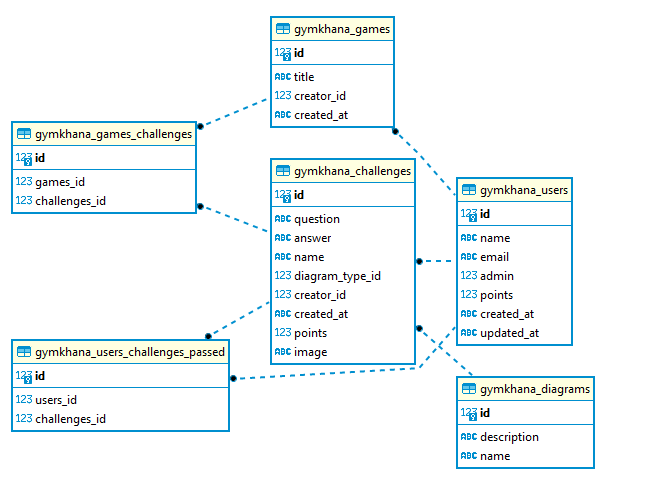
\includegraphics[width=16cm, keepaspectratio]{img/gymkhana_ER.png}
	\caption{Diagrama entidad-relación de la aplicación Ghymkhana App.}\label{fig:diagarma_ER}
\end{figure}



%%%%%%%%%%%%%%%%%%%%%%%%%%%%%%%%%%%%%%%%%%%%%%%%%%%%%%%%%%%%%%%%%%%%%%%%%%%%%%%%
%%%%%%%%%%%%%%%%%%%%%%%%%%%%%%%%%%%%%%%%%%%%%%%%%%%%%%%%%%%%%%%%%%%%%%%%%%%%%%%%
% EXPERIMENTOS Y VALIDACIÓN %
%%%%%%%%%%%%%%%%%%%%%%%%%%%%%%%%%%%%%%%%%%%%%%%%%%%%%%%%%%%%%%%%%%%%%%%%%%%%%%%%

\cleardoublepage

\chapter{Experimentos y validación}

Este capítulo se introdujo como requisito en 2019. 
Describe los experimentos y casos de test que tuviste que implementar para validar tus resultados. 
Incluye también los resultados de validación que permiten afirmar que tus resultados son correctos. 


%%%%%%%%%%%%%%%%%%%%%%%%%%%%%%%%%%%%%%%%%%%%%%%%%%%%%%%%%%%%%%%%%%%%%%%%%%%%%%%%
%%%%%%%%%%%%%%%%%%%%%%%%%%%%%%%%%%%%%%%%%%%%%%%%%%%%%%%%%%%%%%%%%%%%%%%%%%%%%%%%
% RESULTADOS %
%%%%%%%%%%%%%%%%%%%%%%%%%%%%%%%%%%%%%%%%%%%%%%%%%%%%%%%%%%%%%%%%%%%%%%%%%%%%%%%%

\cleardoublepage
\chapter{Resultados}

En este capítulo se incluyen los resultados de tu trabajo fin de grado.

Si es una herramienta de análisis lo que has realizado, aquí puedes poner ejemplos de haberla utilizado para que se vea su utilidad.


%%%%%%%%%%%%%%%%%%%%%%%%%%%%%%%%%%%%%%%%%%%%%%%%%%%%%%%%%%%%%%%%%%%%%%%%%%%%%%%%
%%%%%%%%%%%%%%%%%%%%%%%%%%%%%%%%%%%%%%%%%%%%%%%%%%%%%%%%%%%%%%%%%%%%%%%%%%%%%%%%
% CONCLUSIONES %
%%%%%%%%%%%%%%%%%%%%%%%%%%%%%%%%%%%%%%%%%%%%%%%%%%%%%%%%%%%%%%%%%%%%%%%%%%%%%%%%

\cleardoublepage
\chapter{Conclusiones}
\label{chap:conclusiones}


\section{Consecución de objetivos}
\label{sec:consecucion-objetivos}

Esta sección es la sección espejo de las dos primeras del capítulo de objetivos, donde se planteaba el objetivo general y se elaboraban los específicos.

Es aquí donde hay que debatir qué se ha conseguido y qué no. 
Cuando algo no se ha conseguido, se ha de justificar, en términos de qué problemas se han encontrado y qué medidas se han tomado para mitigar esos problemas.

Y si has llegado hasta aquí, siempre es bueno pasarle el corrector ortográfico, que las erratas quedan fatal en la memoria final.
Para eso, en Linux tenemos aspell, que se ejecuta de la siguiente manera desde la línea de \emph{shell}:

\begin{verbatim}
  aspell --lang=es_ES -c memoria.tex
\end{verbatim}

\section{Aplicación de lo aprendido}
\label{sec:aplicacion}

Aquí viene lo que has aprendido durante el Grado/Máster y que has aplicado en el TFG/TFM. Una buena idea es poner las asignaturas más relacionadas y comentar en un párrafo los conocimientos y habilidades puestos en práctica.

\begin{enumerate}
  \item a
  \item b
\end{enumerate}


\section{Lecciones aprendidas}
\label{sec:lecciones_aprendidas}

Aquí viene lo que has aprendido en el Trabajo Fin de Grado/Máster.

\begin{enumerate}
  \item Aquí viene uno.
  \item Aquí viene otro.
\end{enumerate}


\section{Trabajos futuros}
\label{sec:trabajos_futuros}

Ningún proyecto ni software se termina, así que aquí vienen ideas y funcionalidades que estaría bien tener implementadas en el futuro.

Es un apartado que sirve para dar ideas de cara a futuros TFGs/TFMs.


%%%%%%%%%%%%%%%%%%%%%%%%%%%%%%%%%%%%%%%%%%%%%%%%%%%%%%%%%%%%%%%%%%%%%%%%%%%%%%%%
%%%%%%%%%%%%%%%%%%%%%%%%%%%%%%%%%%%%%%%%%%%%%%%%%%%%%%%%%%%%%%%%%%%%%%%%%%%%%%%%
% APÉNDICE(S) %
%%%%%%%%%%%%%%%%%%%%%%%%%%%%%%%%%%%%%%%%%%%%%%%%%%%%%%%%%%%%%%%%%%%%%%%%%%%%%%%%

\cleardoublepage
\appendix
\chapter{Manual de usuario}
\label{app:manual}

A pesar de haber planificado esta aplicación con esquemas muy sencillos, botones grandes de colores vistosos y claros, debido a que principalmente está enfocada a un público joven e infantil y, que de sobra puede ser entendida sin mayor complejidad por cualquier persona adulta, se deja aquí un pequeño manual de usuario con las principales funcionalidades de la aplicación. \\

\section{Página principal}
La página principal, también comúnmente conocida como \emph{home}. Tiene la única función de presentar la aplicación de manera clara y limpia, con no demasiada información para no bombardear ni agobiar a los potenciales usuarios que puedan visitar la página. En este punto también se exponen dos botones principales que llevan a las dos principales funcionalidades de la aplicación: empezar a jugar y poder registrarse para acceder a las funcionalidades que permiten crear nuevos retos y juegos. 

\begin{figure}
	\centering
	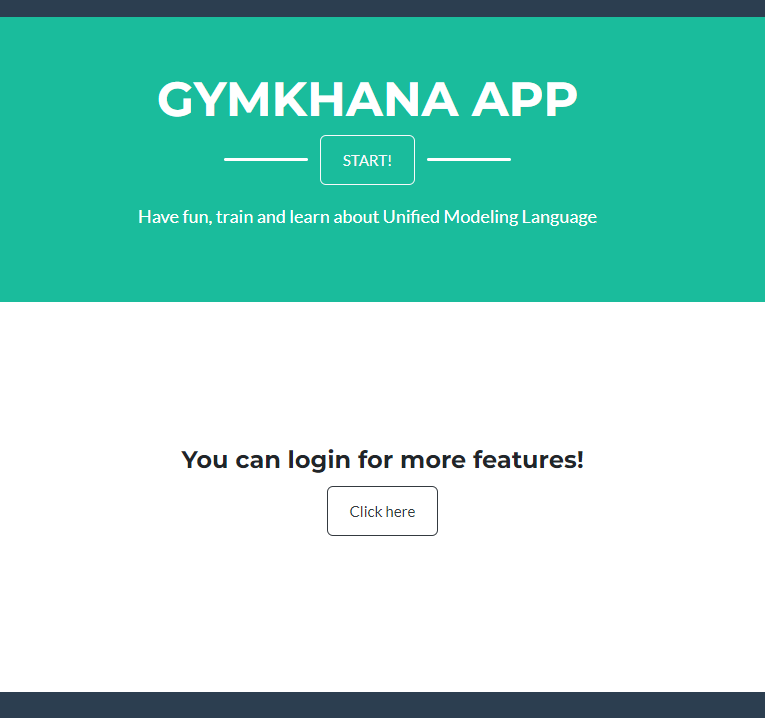
\includegraphics[width=16cm, keepaspectratio]{img/home_html.png}
	\caption{Página principal de la aplicación.}\label{fig:home}
\end{figure}

\section{Menú de juegos}
El menú de juego es la página a la que accedes inmediatamente después de pulsar el botón \emph{START!} de la página principal. Aquí se presentan en manera de lista descendiente todos los juegos subidos a la aplicación. Pulsando sobre la imagen de cada uno de los juegos la aplicación debería llevar al usuario al primer reto de cada una de las pruebas. 

\begin{figure}
	\centering
	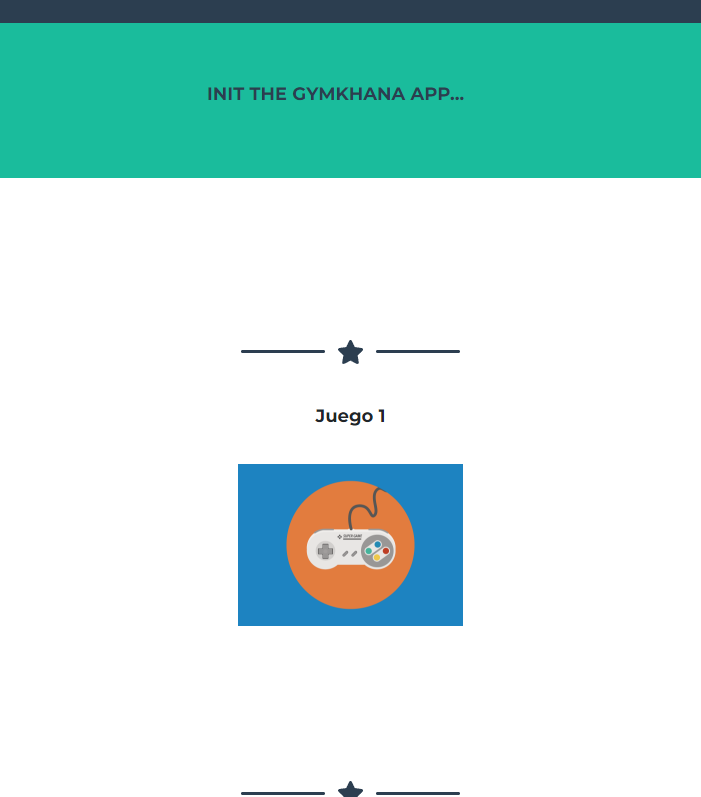
\includegraphics[width=16cm, keepaspectratio]{img/start_html.png}
	\caption{Menú de juegos de la aplicación.}\label{fig:start}
\end{figure}

\section{Página de los retos}
Una vez pulsado sobre uno de los juegos redirigirá al usuario a la página con el primer reto del juego seleccionado. Todos los retos siguen el mismo esquema: 
\begin{enumerate}
	\item En la cabecera del reto se ve el nombre del tipo de diagrama UML con el que está relacionado el reto.
	\item Para abrir el reto tenemos un pequeño resumen explicando el tipo de diagrama que es, y para que sirve. 
	\item Luego se plantea la pregunta o tarea que debe responder el usuario para poder completar el reto. 
	\item Debajo está la imagen con el diagrama UML sobre el cual el usuario debe extrae la información para poder contestar el reto.
	\item Por último un cuadro de texto y un botón de enviar la respuesta. 
\end{enumerate}
Después de enviar la respuesta el usuario es redirigido a otra página donde se le dice al usuario si la respuesta es correcta o no. En caso de que sea correcto el usuario podrá continuar con el siguiente reto, en caso de que el juego contenga más y en caso de que sea incorrecta se le da la opción de volver al menú de juegos o volver a intentar el reto fallado. 
\begin{figure}
	\centering
	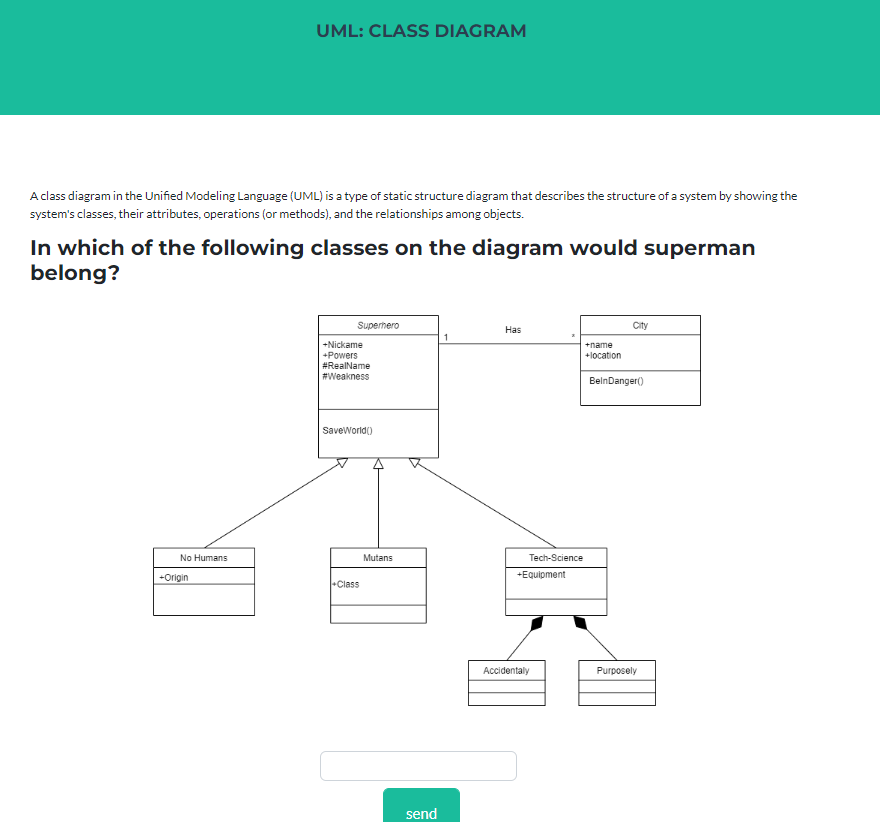
\includegraphics[width=16cm, keepaspectratio]{img/challenge_html.png}
	\caption{Página de retos.}\label{fig:challenge}
\end{figure}

\section{Inicio de sesión}
La sección de inicio de sesión se reduce a un simple \emph{login}. Por motivos de seguridad no se ha implementado las funcionalidades de registro o dar de alta a un nuevo usuario. El uso es simple; el usuario debe introducir las credenciales dadas por el administrador de la aplicación y pulsar el botón de iniciar sesión. 
\begin{figure}
	\centering
	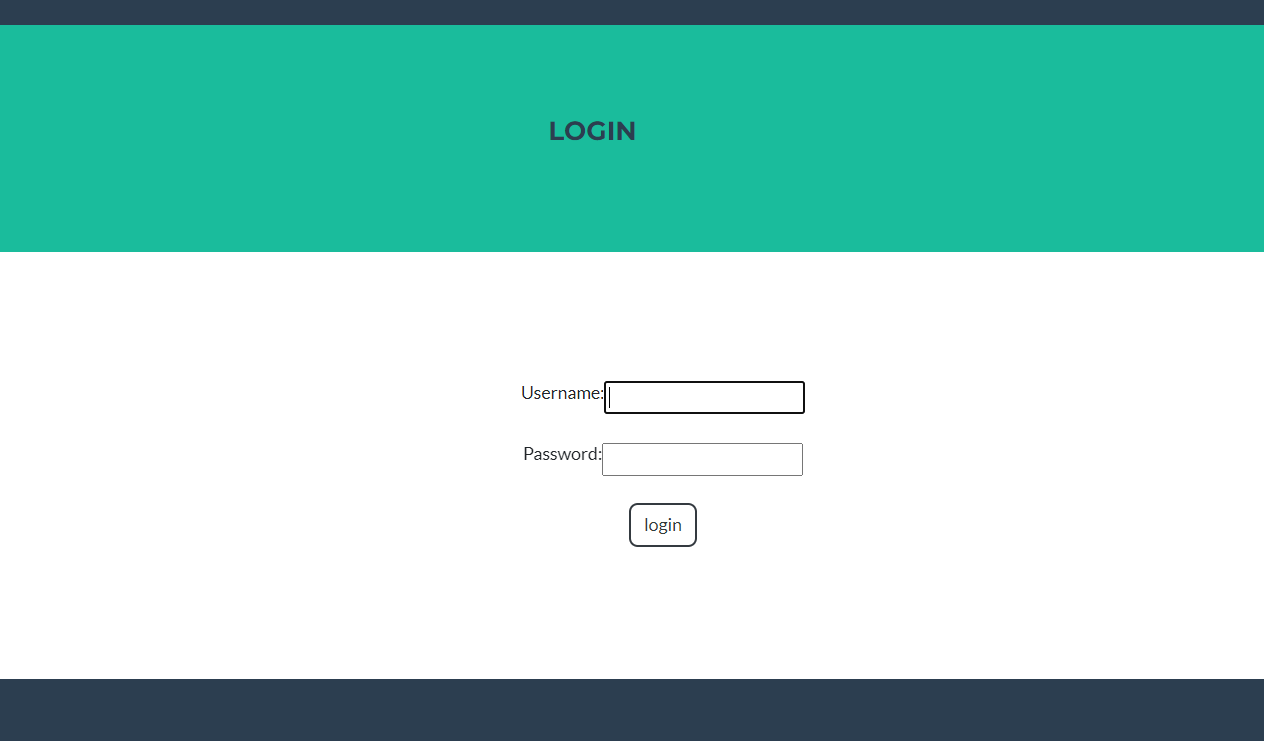
\includegraphics[width=16cm, keepaspectratio]{img/login_html.png}
	\caption{Menú de juegos de la aplicación.}\label{fig:login}
\end{figure}

\section{Perfil del usuario}
Una vez se ha iniciado sesión y el usuario está registrado se accede al perfil. Dentro de este encontrarás los puntos acumulados por haber superado retos y acceso a varias funciones. Desde este punto es el único punto desde el cual puedes acceder a poder subir retos y poder crear juegos. En la parte inferior está el botón para poder cerrar sesión y volver a la aplicación como usuario anónimo. 
\begin{figure}
	\centering
	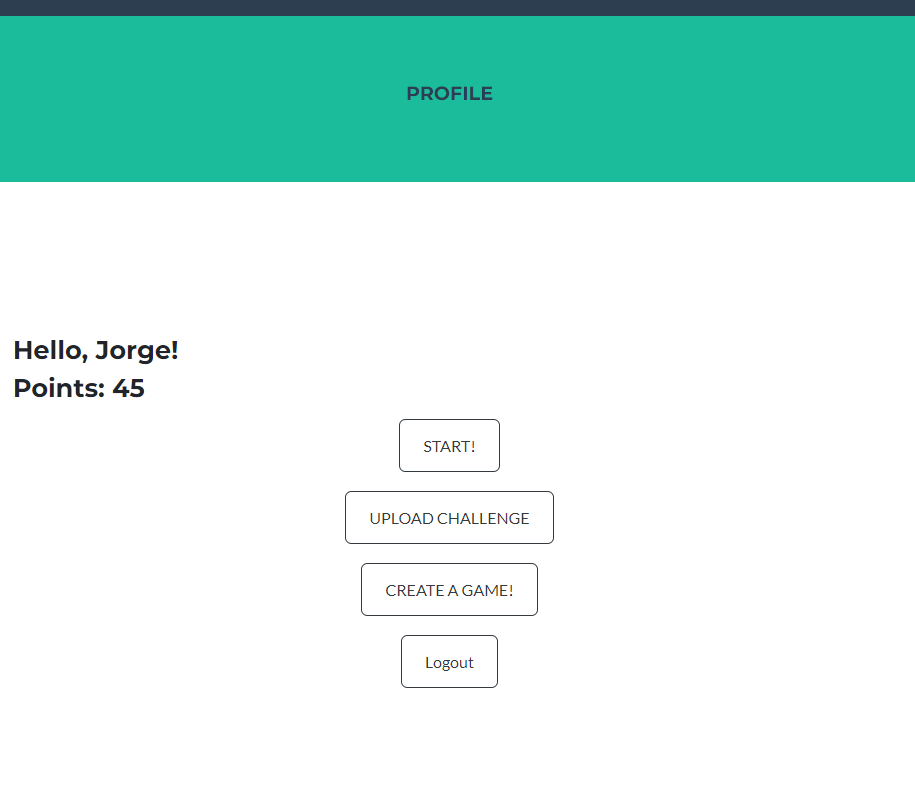
\includegraphics[width=16cm, keepaspectratio]{img/profile_html.png}
	\caption{Menú de juegos de la aplicación.}\label{fig:profile}
\end{figure}

\section{Subida de retos}
Si el usuario ha accedido hasta la página de subida de retos para poder continuar deberá rellenar el formulario. Se supone que esta funcionalidad solo se le concede a usuarios de confianza, por tanto aunque el formulario si que sea resistente a intentos de subida con campos vacíos, no está diseñado para comprobar que los campos rellenos sean coherentes con lo que se espera recibir. Se asume que el usuario al que se le han concedido estos permisos subirá retos coherentes y de manera responsable. También hay que tener en cuenta que en este punto se pueden subir imágenes que se guardan directamente en la máquina que hospeda la web en Heroku, por tanto si esto estuviera abierto al público en general se podría generar un sobrecarga de memoria en la maquina que hospeda la web.
El formulario es bastante claro con los campos a rellenar, la imagen la debemos seleccionar haciendo click en el campo que pide la misma, y subiendo la imagen deseada desde la memoria del ordenador desde el que se esté haciendo la solicitud. 
Para completar con la subida solo hay que pulsar el botón situado al final de la página. 

\begin{figure}
	\centering
	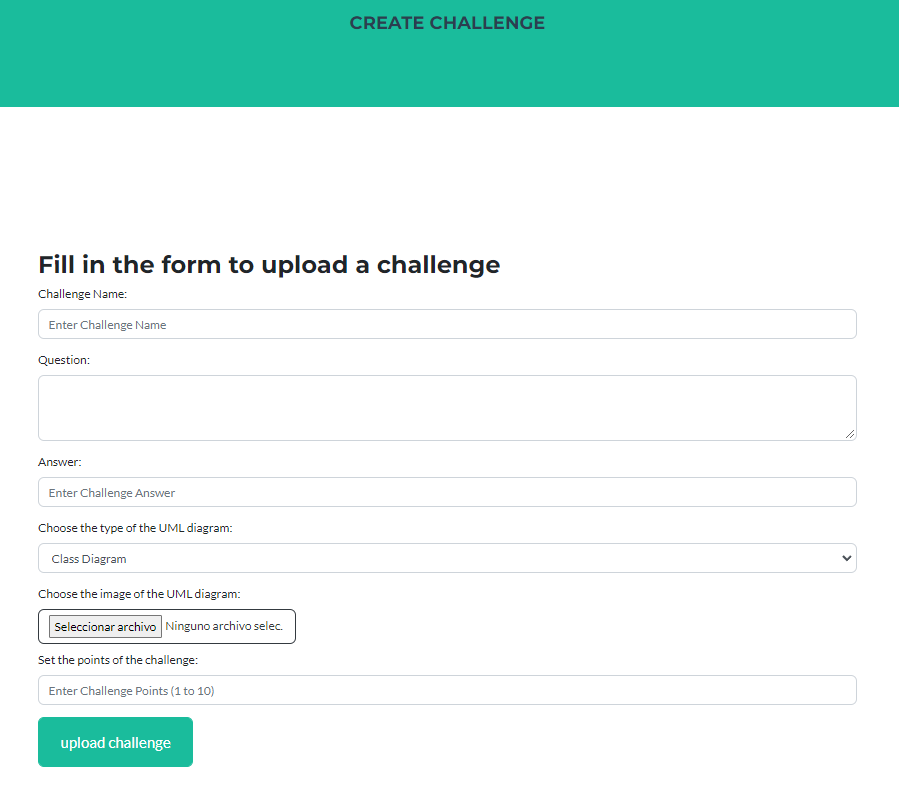
\includegraphics[width=16cm, keepaspectratio]{img/create_challenge_html.png}
	\caption{Menú de juegos de la aplicación.}\label{fig:create_challenge}
\end{figure}

\section{Creación de juegos}

\begin{figure}
	\centering
	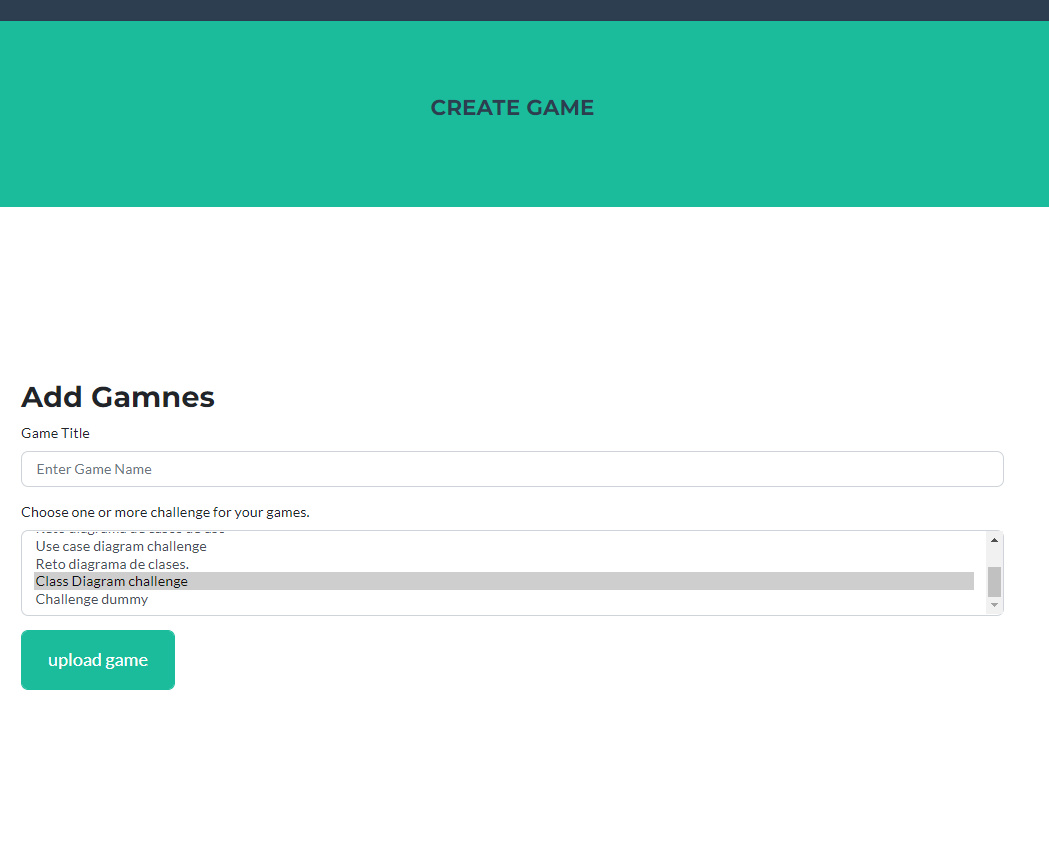
\includegraphics[width=16cm, keepaspectratio]{img/create_game_html.png}
	\caption{Menú de juegos de la aplicación.}\label{fig:create_game}
\end{figure}


\chapter{Anexo II: Ejemplos de Diagramas UML}
\label{app:diagramas}
% Contenido del anexo II

\section{Diagrama de clases}
En este diagrama de clases, hay una clase padre y dos clases hijas. En este caso la clase padre cuenta con unos atributos y métodos comunes, los cuales comparte con las clases hijas. Las clases hijas en cambio tienen cada una unos atributos y métodos que no pueden compartir entre ellas ni con la clase padre.
\begin{figure}
	\centering
	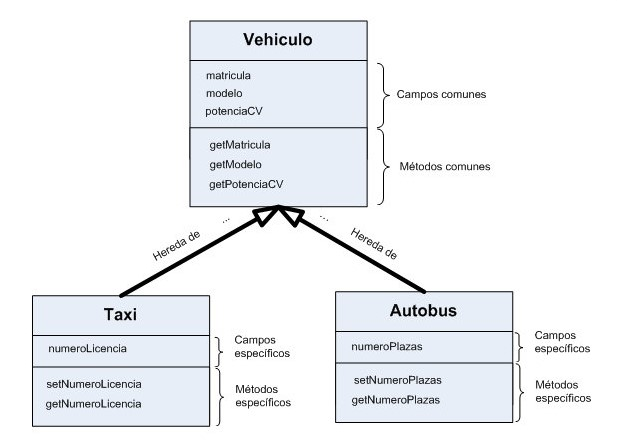
\includegraphics[width=14cm, keepaspectratio]{img/diagrama_clases.png}
	\caption{Ejemplo de diagrama de clases.}\label{fig:diagrama_clases}
\end{figure}

\section{Diagrama de objetos}
Los diagrama de objetos están fuertemente relacionados con los diagramas de clases, tanto es así que hasta comparten símbolos y figuras. Básicamente para seguir con el objeto anterior de los vehículos, en este ejemplo se puede ver los datos o "fotografía" de un objeto del sistema en un momento determinado del tiempo. 
\begin{figure}
	\centering
	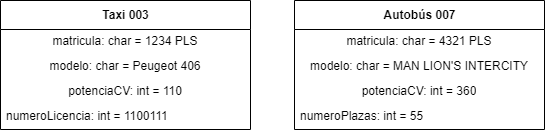
\includegraphics[width=14cm, keepaspectratio]{img/diagrama_objetos.png}
	\caption{Ejemplo de diagrama de objetos.}\label{fig:diagrama_objetos}
\end{figure}

\section{Diagrama de despliegue}
Este diagrama de despliegue modela la arquitectura en tiempo de ejecución de un sistema. Se muestra la configuración de los elementos de hardware, identificados como nodos. Y muestra la trazas de elementos y artefactos del software en estos nodos. 
\begin{figure}
	\centering
	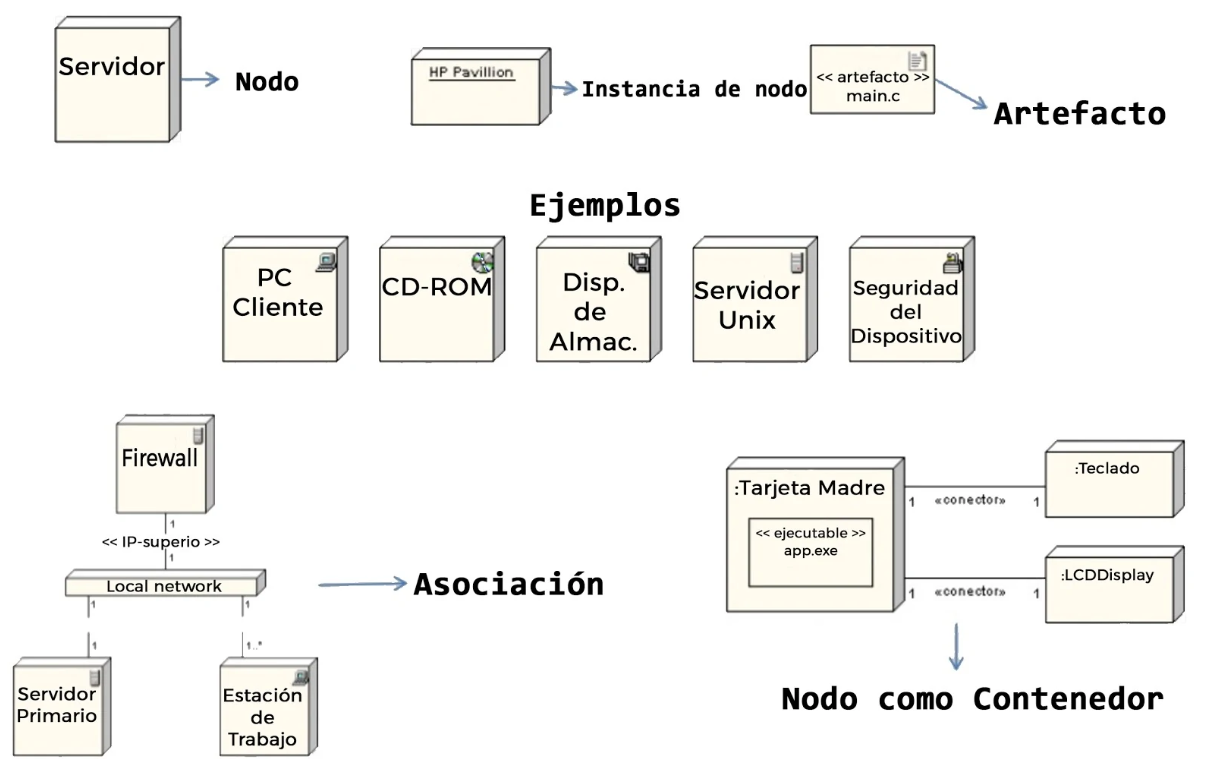
\includegraphics[width=16cm, keepaspectratio]{img/diagrama_despliegue.png}
	\caption{Ejemplo de diagrama de despliegue.}\label{fig:diagrama_despliegue}
\end{figure}

\section{Diagrama de componentes}
En este diagrama de componentes se puede visualizar la estructura y la funcionalidad de un software de correo electrónico. Muestra la interacción a través de sus tres interfaces. La linea discontinua etiquetada con "use" indica que el usuario es dependiente de esa interfaz (management port) para supervisar y administrar el correcto funcionamiento del sistema.
\begin{figure}
	\centering
	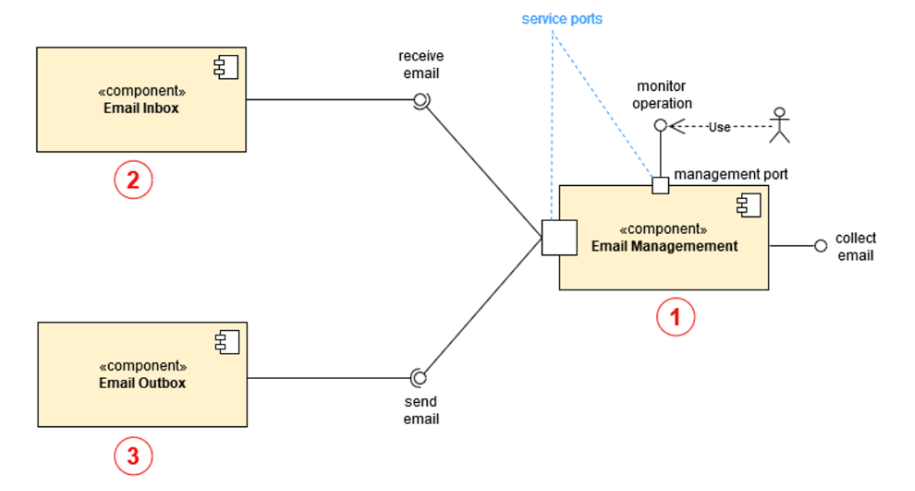
\includegraphics[width=18cm, keepaspectratio]{img/diagrama_componentes.png}
	\caption{Ejemplo diagrama de componentes.}\label{fig:diagrama_componentes}
\end{figure}

\section{Diagrama de paquetes}
En este ejemplo de diagrama de paquetes tiene la intención de mostrar la organización y disposición de los diferentes elementos que componen un aplicación web para compras. Las carpetas representa la anidación de elementos del software, y estas a la vez se organizan jerárquicamente dentro del diagrama. 
\begin{figure}
	\centering
	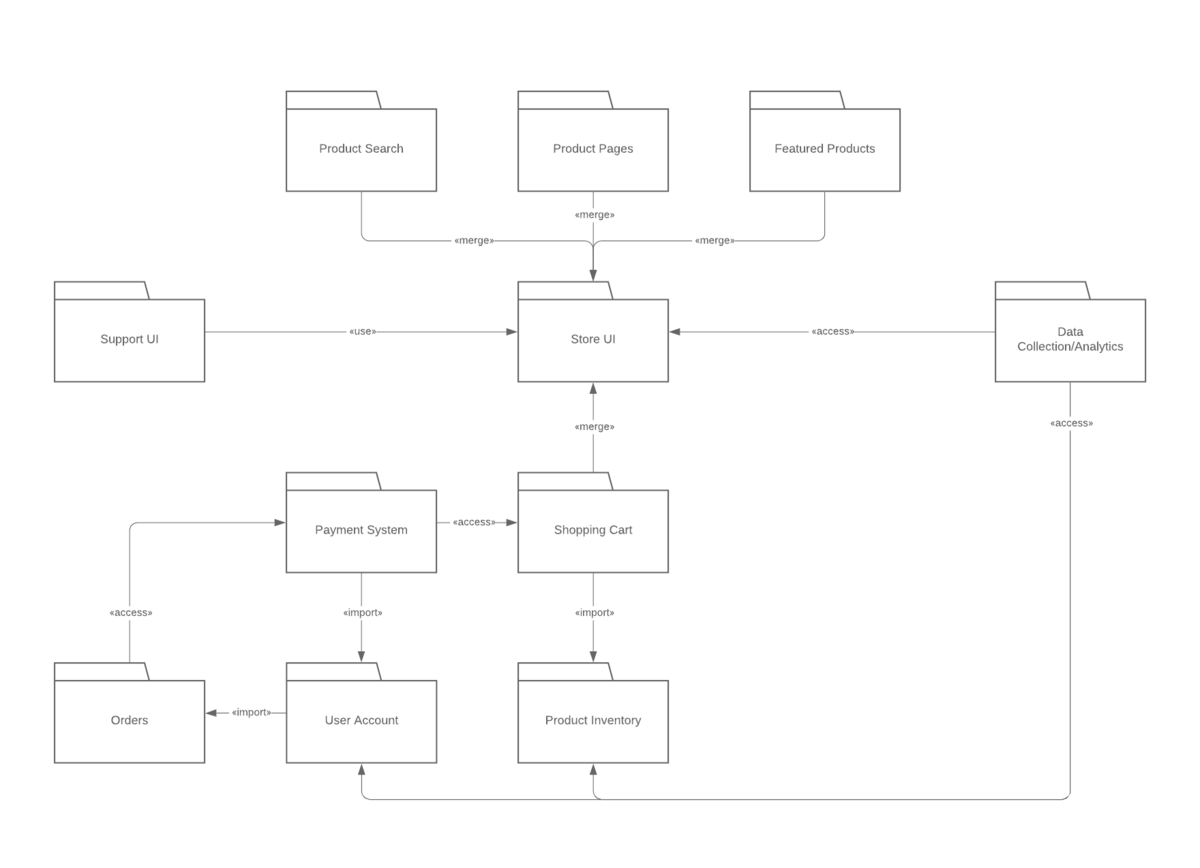
\includegraphics[width=14cm, keepaspectratio]{img/diagrama_paquetes.png}
	\caption{Ejemplo diagrama de paquetes.}\label{fig:diagrama_paquetes}
\end{figure}

\section{Diagrama de estructura compuesta}
En este ejemplo podemos apreciar el diagrama de estructura compuesta de un sistema contraincendios. Se puede ver que la unidad central de control está compuesta por componentes más pequeños (sirena, aspersores, sensores, monitores...), que a su vez pertenecen al sistema general.
\begin{figure}
	\centering
	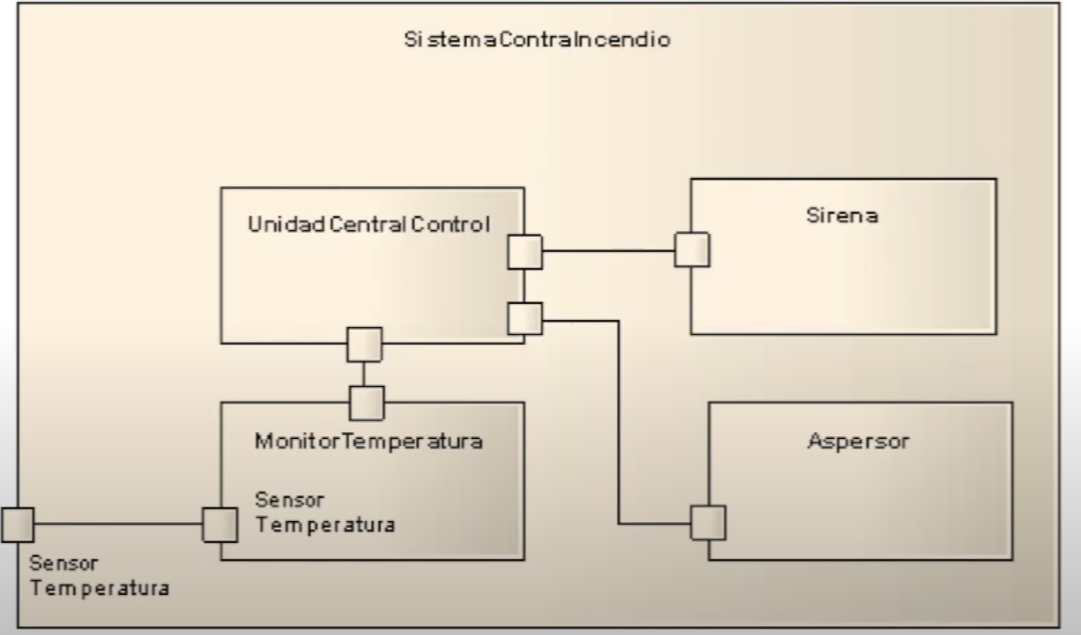
\includegraphics[width=12cm, keepaspectratio]{img/diagrama_estructura_compuesta.png}
	\caption{Ejemplo diagrama de estructura compuesta.}\label{fig:diagrama_estructura_compuesta}
\end{figure}

\section{Diagrama de actividad}
Este ejemplo de diagrama es uno de los usados para los retos de Gymkhana App. Este tipo de diagramas es de los más conocidos, en este caso se trata de seguir el flujo de trabajo, pudiendo actuar de distinta manera dependiendo de las respuestas del sistema a diferentes preguntas (representadas con rombos). 
\begin{figure}
	\centering
	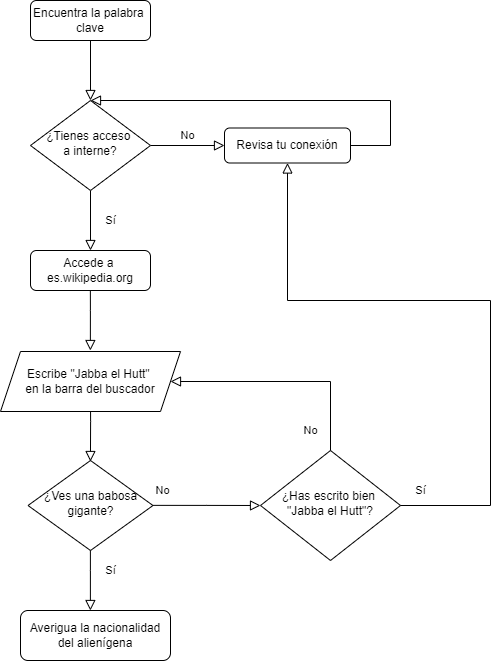
\includegraphics[width=10cm, keepaspectratio]{img/diagrama_actividad.png}
	\caption{Ejemplo diagrama de actividad.}\label{fig:diiagrama_actividad}
\end{figure}

\section{Diagrama de casos de uso}
Este ejemplo modela la funcionalidad de un "Sistema Apocalipsis Zombie" con los diferentes casos de uso representado con elipses. Se muestra también la interacción que tiene el actor (superviviente) con el sistema. Este diagrama ha sido diseñado para uno de los primeros retos de la aplicación Gymkhana App.
\begin{figure}
	\centering
	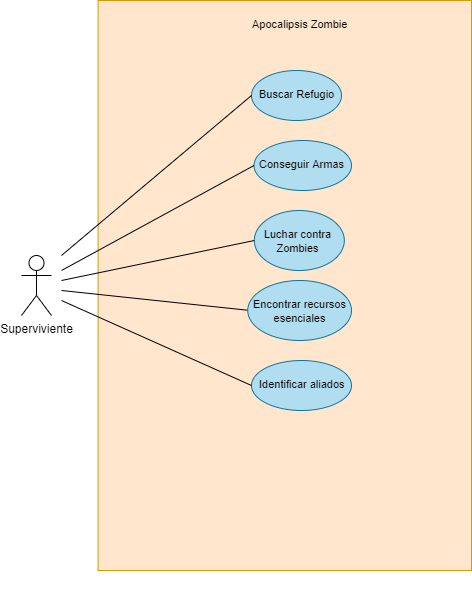
\includegraphics[height=18cm,width=12cm, keepaspectratio]{img/diagrama_casos_uso.png}
	\caption{Ejemplo diagrama casos de uso.}\label{fig:diagrama_casos_uso}
\end{figure}

\section{Diagrama de máquina de estados}
En este ejemplo se muesta un diagrama del proceso de inscripción y finalización de una asignatura de la universidad. Se puede como el estado pasa de tratar de apuntarse a una asignatura, poder matricularte en esta y pasar los exámenes finales. 
\begin{figure}
	\centering
	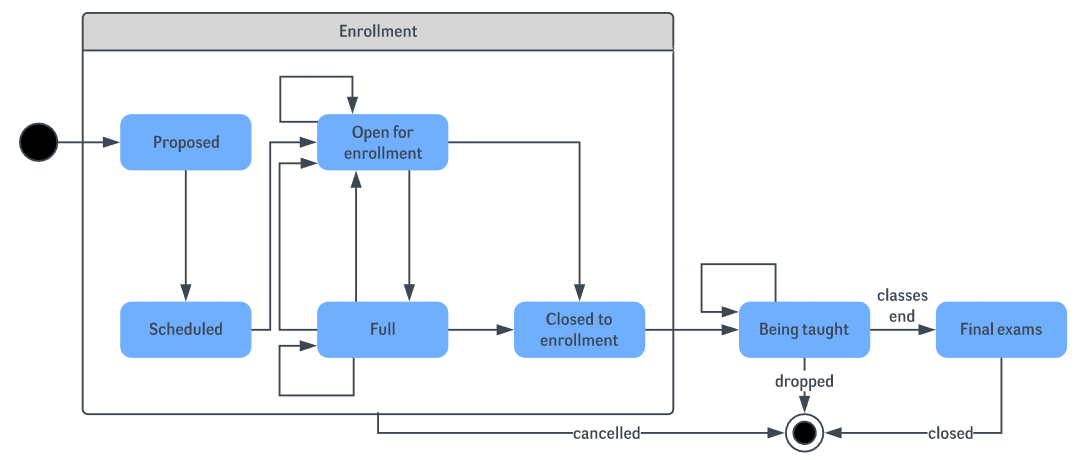
\includegraphics[width=16cm, keepaspectratio]{img/diagrama_maquina_estados.png}
	\caption{Ejemplo diagrama de máquina de estados.}\label{fig:diagrama_maquina_estados}
\end{figure}

\section{Diagrama de interacción}
Como dentro de estos tipos de diagramas se pueden clasificar cuatro más, en este apartado se aportan ejemplos sencillos de alguno de ellos.

Los diagramas de colaboración se centran en los aspectos estructurales y la arquitectura de los objetos de un software. En el ejemplo se muestra el flujo de organización de una tienda online, con el tipo de mensajes y de llamadas que se hacen entre los objetos del sistema. 
\begin{figure}
	\centering
	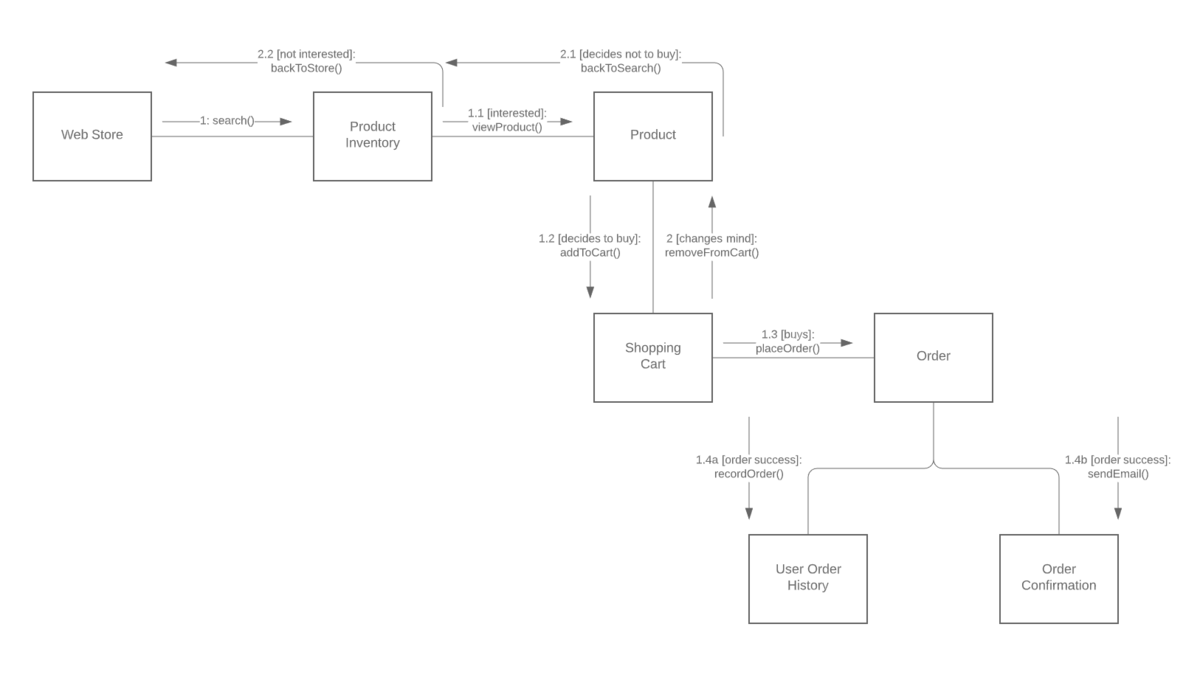
\includegraphics[width=14cm, keepaspectratio]{img/diagrama_colaboracion.png}
	\caption{Ejemplo diagrama de colaboración}\label{fig:diagrama_colaboracion}
\end{figure}

Los diagramas de secuencia se centrar en representa las interacciones entre los eventos de un sistema. En el ejemplo se muestra la secuencia de eventos de un software de manejo de una agenda, enlazada a una dirección de correo electrónico.
\begin{figure}
	\centering
	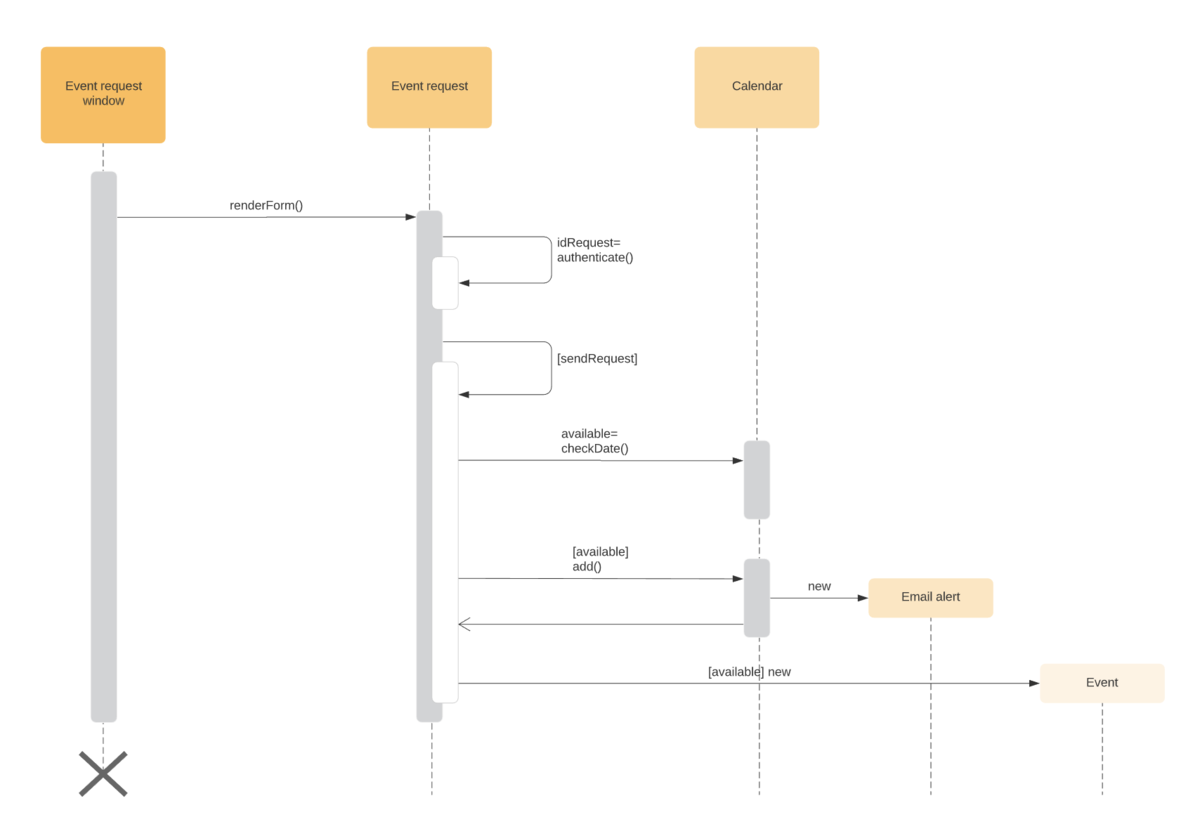
\includegraphics[width=14cm, keepaspectratio]{img/diagrama_secuencia.png}
	\caption{Ejemplo diagrama de secuencia}\label{fig:diagrama_secuencia}
\end{figure}

Los diagramas de tiempos se unas para representar la línea de vida de un objeto en una instancia y en el tiempo. Se representa los cambios con nivel alto y bajo con señales. En el ejemplo se puede ver un diagrama del comportamiento de los objetos que forman una sistema contraincendios.
\begin{figure}
	\centering
	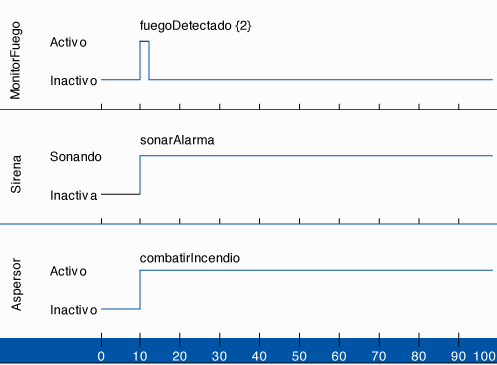
\includegraphics[width=12cm, keepaspectratio]{img/diagrama_tiempos.png}
	\caption{Ejemplo diagrama de tiempos.}\label{fig:diagrama_tiempos}
\end{figure}

%\cleardoublepage


%%%%%%%%%%%%%%%%%%%%%%%%%%%%%%%%%%%%%%%%%%%%%%%%%%%%%%%%%%%%%%%%%%%%%%%%%%%%%%%%
%%%%%%%%%%%%%%%%%%%%%%%%%%%%%%%%%%%%%%%%%%%%%%%%%%%%%%%%%%%%%%%%%%%%%%%%%%%%%%%%
% BIBLIOGRAFIA %
%%%%%%%%%%%%%%%%%%%%%%%%%%%%%%%%%%%%%%%%%%%%%%%%%%%%%%%%%%%%%%%%%%%%%%%%%%%%%%%%

\cleardoublepage

% Las siguientes dos instrucciones es todo lo que necesitas
% para incluir las citas en la memoria
\bibliographystyle{abbrv}
\bibliography{memoria}  % memoria.bib es el nombre del fichero que contiene
% las referencias bibliográficas. Abre ese fichero y mira el formato que tiene,
% que se conoce como BibTeX. Hay muchos sitios que exportan referencias en
% formato BibTeX. Prueba a buscar en http://scholar.google.com por referencias
% y verás que lo puedes hacer de manera sencilla.
% Más información: 
% http://texblog.org/2014/04/22/using-google-scholar-to-download-bibtex-citations/

%https://es.wikipedia.org/wiki/Lenguaje_unificado_de_modelado
%versiones uml https://www.omg.org/spec/UML/
%https://www.omg.org/spec/UML/2.5.1/PDF
%https://docs.djangoproject.com/en/3.2/
%https://www.uml-diagrams.org/uml-25-diagrams.html
%https://www.lucidchart.com/pages/es/diagrama-de-interaccion-uml

\end{document}
